% Manual de usuario
% Modificado por Crisostomo Barajas a partir del manual creado por Emmanuel Martinez
% Julio 2022

\documentclass[12pt,twoside,letter]{ol-softwaremanual}
\usepackage{float}
\usepackage[utf8]{inputenc}
\usepackage[a4paper,width=160mm,top=25mm,bottom=25mm]{geometry}
\usepackage[lining,tabular]{fbb} % so math uses tabular lining figures
\usepackage{graphicx}
\usepackage{enumitem}
\setlist{leftmargin=*}
\usepackage{listings}
\lstset{basicstyle=\ttfamily,frame=single,xleftmargin=3em,xrightmargin=3em}
\usepackage[os=win]{menukeys}
\renewmenumacro{\keys}[+]{shadowedroundedkeys}
\usepackage{framed}
\usepackage{etoolbox}
\AtBeginEnvironment{leftbar}{\sffamily\small}
\usepackage{array,lipsum}
\newenvironment{fulltable}[1][H]
 {\begin{table}[#1]%
  \hspace*{-\leftmarginwidth}%
  \begin{minipage}{\fullwidth}}
 {\end{minipage}\end{table}}
\usetikzlibrary{chains,arrows,shapes,positioning}
\usepackage{hyperref}
\graphicspath{{figures/}} %Setting the graphicspath
\renewcommand\abstractname{Introduction}

\usepackage[spanish]{babel}

\usepackage{multicol}

\usepackage{caption}
\usepackage[rightcaption]{sidecap}
\usepackage{subcaption}
\usepackage{wrapfig}
\usepackage{pifont}
\usepackage{fontawesome}

\usepackage{amsmath}
\usepackage{amssymb}

\usepackage{fancyhdr}

\pagestyle{fancy}
\fancyhf{}
\fancyhead[LE,RO]{{\footnotesize HDSP - UIS}}
\fancyhead[RE,LO]{{\footnotesize ReDs - Manual de Usuario}}
\fancyfoot[CE,CO]{\thepage}
%\fancyfoot[LE,RO]{\thepage}

\definecolor{ClearPurple}{RGB}{136, 0, 255}

\usepackage{tikz}
\newcommand*\circled[1]{\tikz[baseline=(char.base)]{
            \node[shape=circle,draw,inner sep=2pt] (char) {#1};}}

\newenvironment{Figure}
  {\par\medskip\noindent\minipage{\linewidth}}
  {\endminipage\par\medskip}
  
%\setlength{\parskip}{2em}
\setlength{\parskip}{6pt}%
\setlength{\parindent}{0pt}%
\setlength{\itemsep}{0em}

\title{\large{Manual de Usuario}\\ \vspace{10mm} \huge{Reconstrucción de Datos Sísmicos}\\ \vspace{5mm} \huge{ReDs}}
\author{
\includegraphics[width=14cm]{figures/all_logos3.png} \\ Emmanuel Martínez \\ Crisóstomo A. Barajas-Solano}
\softwarelogo{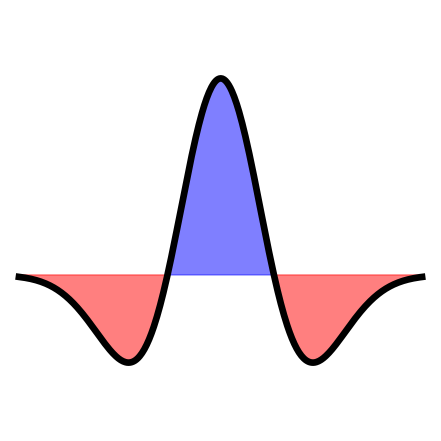
\includegraphics[width=7cm]{figures/icon}}
\version{2022.10}



\begin{document}

\maketitle

\newpage\null\thispagestyle{empty}\newpage

\begin{center}
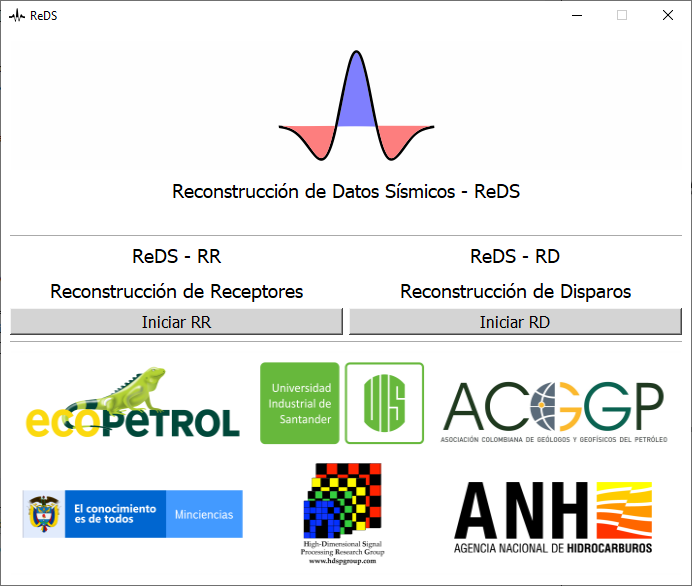
\includegraphics[width=.65\linewidth]{launch.png}
\end{center}
\begin{abstract}
%\includegraphics[width=1.0\linewidth]{PhysLogger.png}\\
%Esta aplicación pertenece al proyecto de investigación 9836, de la Universidad Industrial de Santander, Colombia. Esta aplicación permite la reconstrucción de trazas de muestras sísmicas mediante 4 diferentes algoritmos. Esta reconstrucción puede ser configurada por el usuario de tal manera que pueda realizar diferentes tipos de submuestreo y ajuste de parámetros mediante una interfaz gráfica de usuario.
La herramienta software Reconstrucción de Datos Sísmicos - ReDs hace parte del proyecto 9836 - ``Nuevas tecnologías computacionales para el diseño de sistemas de adquisición sísmica 3D terrestre con muestreo compresivo para la reducción de costos económicos e impactos ambientales en la exploración de hidrocarburos en cuencas terrestres colombianas''.

El proyecto 9836 está adscrito a la Convocatoria para la financiación de proyectos de investigación en geociencias para el sector de hidrocarburos, desarrollado por la alianza Universidad Industrial de Santander (UIS), ECOPETROL y la Asociación Colombiana de Geólogos y Geofísicos del Petróleo (ACGGP). 

Este proyecto es financiado por MINCIENCIAS y la Agencia Nacional de Hidrocarburos (ANH). Los derechos y licencias de uso sobre esta aplicación software están reservados a las entidades aportantes.
\end{abstract}

\newpage\null\thispagestyle{empty}\newpage

\clearpage
\tableofcontents

\clearpage

\newpage\null\thispagestyle{empty}\newpage

\section{Visión General de la Aplicación ReDs}

Esta aplicación Reconstrucción de Datos Sísmicos (ReDs) permite la reconstrucción de receptores y disparos sísmicos. Para esto, la aplicación ReDs dispone de dos modos de operación:
\begin{dingautolist}{192}
	\setlength\itemsep{0em}
	\item Reconstrucción de Receptores (ReDs - RR)
	\item Reconstrucción de Disparos (ReDs - RD)
\end{dingautolist}

\begin{Figure}
	\centering
	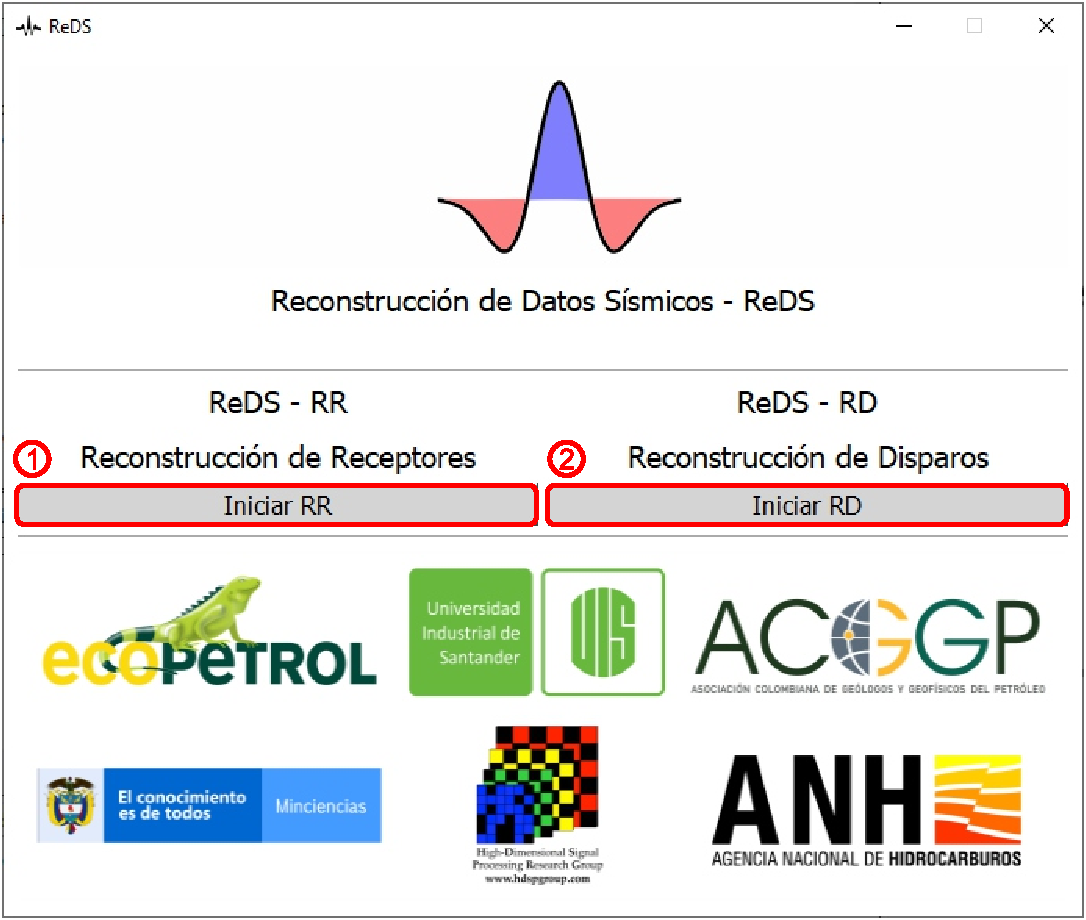
\includegraphics[width=0.65\linewidth]{launch2}
	\captionof{figure}{Secciones de la pantalla de inicio de ReDs.}
	\label{fig:launch}
\end{Figure}

Ambos modos de operación, RR y RD, realizan la reconstrucción de datos sísmicos usando 4 algoritmos numéricos diferentes:
\begin{itemize}[leftmargin=0.5in]
	\setlength\itemsep{0em}
	\item FISTA (Fast Iterative Shrinkage-Thresholding Algorithm): permite resolver problemas inversos lineales mediante un algoritmo iterativo rápido
	\item GAP (Generalized Alternating Projection): resuelve el problema de seguimiento de base grupal, que extiende el seguimiento de base reemplazando la norma $ \ell_1 $ por una norma ponderada $ \ell_{2,1} $.
	\item TwIST (Two-step Iterative Shrinkage/Thresholding): basado en el algoritmo ISTA, permite la resolución de problemas inversos
	\item ADMM (Alternating Direction Method of Multipliers): resuelve problemas de optimización convexos dividiéndolos en partes más pequeñas.
\end{itemize}

El usuario puede configurar cada uno de los algoritmos de reconstrucción de tal manera que pueda realizar diferentes tipos de submuestreo y ajuste de parámetros, todo desde una interfaz gráfica de usuario simple y clara. Aunque los modos de reconstrucción RR y RD presentan diferencias en su operación, están diseñados bajo las mismas directivas. Por esta razón, ambas interfaces gráficas cuentan con varias secciones en común.

La figura \ref{fig:vision} presenta las 7 secciones de la interfaz general del modo Reds - RR, a mencionar:
\begin{dingautolist}{192}
	\setlength\itemsep{0em}
	\item Barra del menú
	\item Lector de datos
	\item Panel de algoritmos
	\item Panel de submuestreo
	\item Menú de experimentos
	\item Menú de cambio de vista
	\item Menú de visualización
\end{dingautolist}

\begin{Figure}
    \centering
    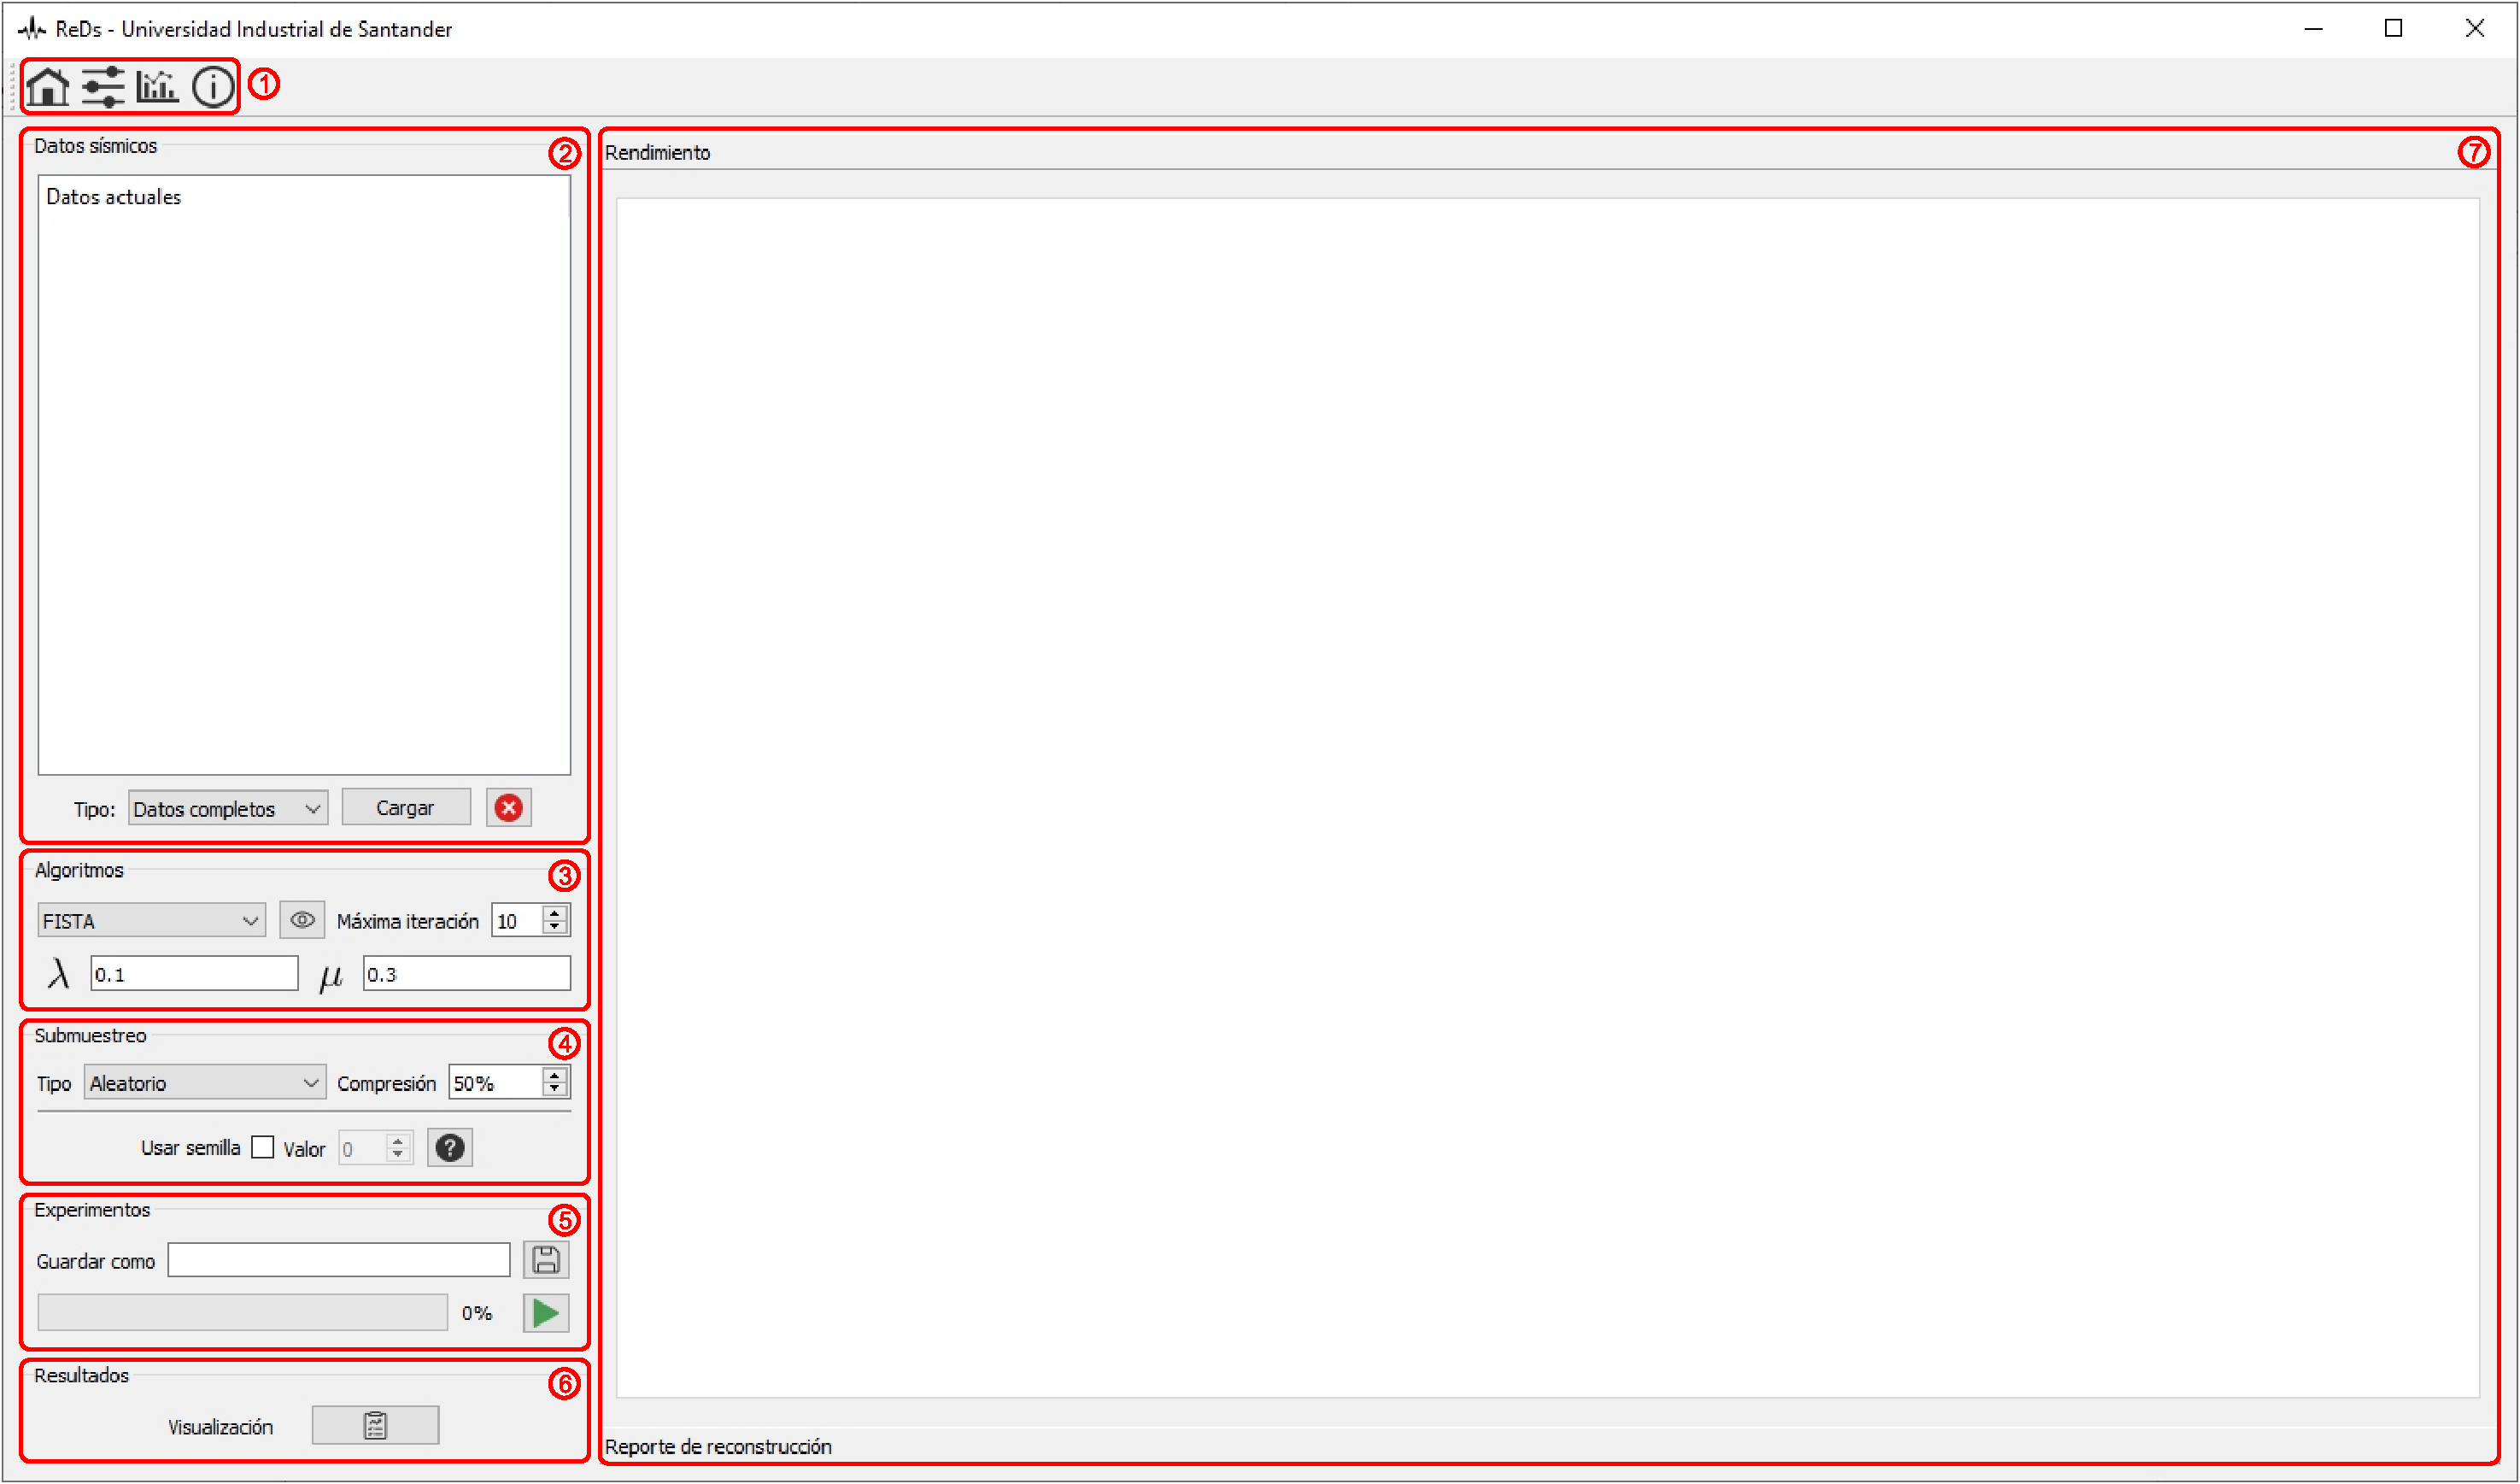
\includegraphics[width=1\linewidth]{figures/vision_v2}
     \captionof{figure}{Secciones de la interfaz general del modo Reds - RR.}
    \label{fig:vision}
\end{Figure}

{\color{red}La figura ToDo presenta las ToDo secciones de la interfaz general del modo ReDs - RD, a mencionar:

ToDo}

\begin{Figure}
	\centering
	
\includegraphics[width=0.75\linewidth]{figures/blank}
	\captionof{figure}{{\color{red}Secciones de la interfaz general del modo Reds - RD.}}
	\label{fig:rd}
\end{Figure}

\newpage
\section{Módulo ReDs - Reconstrucción de Receptores (RR)}

El módulo ReDS-RR (reconstrucción de receptores) realiza la estimación de trazas faltantes en un disparo sísmico, usando algoritmos de gradiente descendiente y aprovechando representaciones escasas de los datos en dominios transformados como Curvelet, DCT y Wavelets.

A continuación se mostrará de forma especifican los modos de uso del módulo ReDs - RR, las diferentes configuraciones y opciones que pueden ser aplicadas a los datos sísmicos para la realización de diferentes tipos de experimentos. Cabe resaltar que de acuerdo al tipo de prueba que se quiera realizar, el comportamiento de los paneles cambiará para adecuarse a dicha tarea.

\subsection{Modo Sencillo}

La aplicación cuenta con una barra de tareas, que se encuentra en la parte superior \circled{1} de la figura \ref{fig:vision}. Aquí se observan 3 botones distintos que permitirán realizar distintos tipos de pruebas sobre los datos sísmicos.

\begin{multicols}{2}

Como se observa en la figura \ref{fig:main_button}, el primer botón habilitará a la aplicación para realizar pruebas generales sobre los datos sísmicos, este es el menú principal.

\begin{Figure}
    \centering
    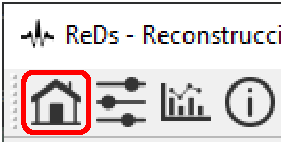
\includegraphics[width=0.4\linewidth]{single-tab}
     \captionof{figure}{Botón del menú principal.}
    \label{fig:main_button}
\end{Figure}

\end{multicols}

El menú principal permite realizar experimentos con los datos sísmicos siguiendo el orden que se observa en la figura \ref{fig:vision}. A continuación se muestra paso a paso el funcionamiento de cada uno los paneles, desde la lectura de datos sísmicos hasta la visualización y guardado de resultados.

\subsubsection{Lectura de Datos}

El panel de lectura de datos \circled{2}, situado al extremo izquierdo superior en la figura \ref{fig:vision}, muestra los nombres de los datos sísmicos que el usuario haya cargado en la aplicación para realizar diversas pruebas.\\

\textbf{Leyendo un dato sísmico} \label{sec:data_lecture}

\begin{multicols}{2}
	
\begin{Figure}
	\centering
	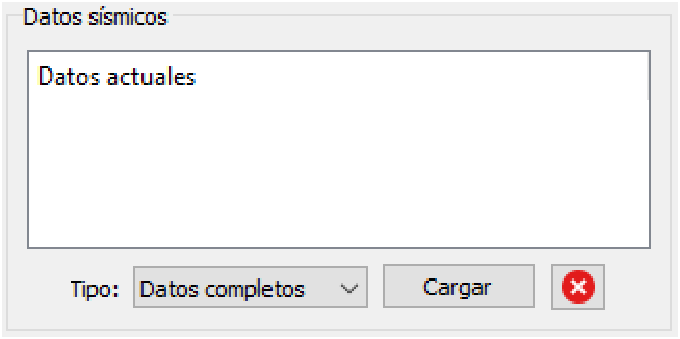
\includegraphics[width=.9\linewidth]{data-lecture-1.pdf}
	\captionof{figure}{Cargando un dato sísmico.}
	\label{fig:data_lecture_1}
\end{Figure}

Para leer un dato sísmico, se pulsa la opción \emph{Cargar} en \circled{2}, como se observa en la figura \ref{fig:data_lecture_1}. Inmediatamente se abrirá la ventana \textit{Abrir dato sísmico}, como se observa en la figura \ref{fig:data_lecture_2}, donde el usuario podrá seleccionar un dato sísmico. Para este ejemplo cargaremos \emph{data.npy}.
La aplicación ReDs reconoce las extensiones \emph{.npy} y \emph{.mat} para cargar datos sísmicos.

\end{multicols}

\begin{Figure}
    \centering
    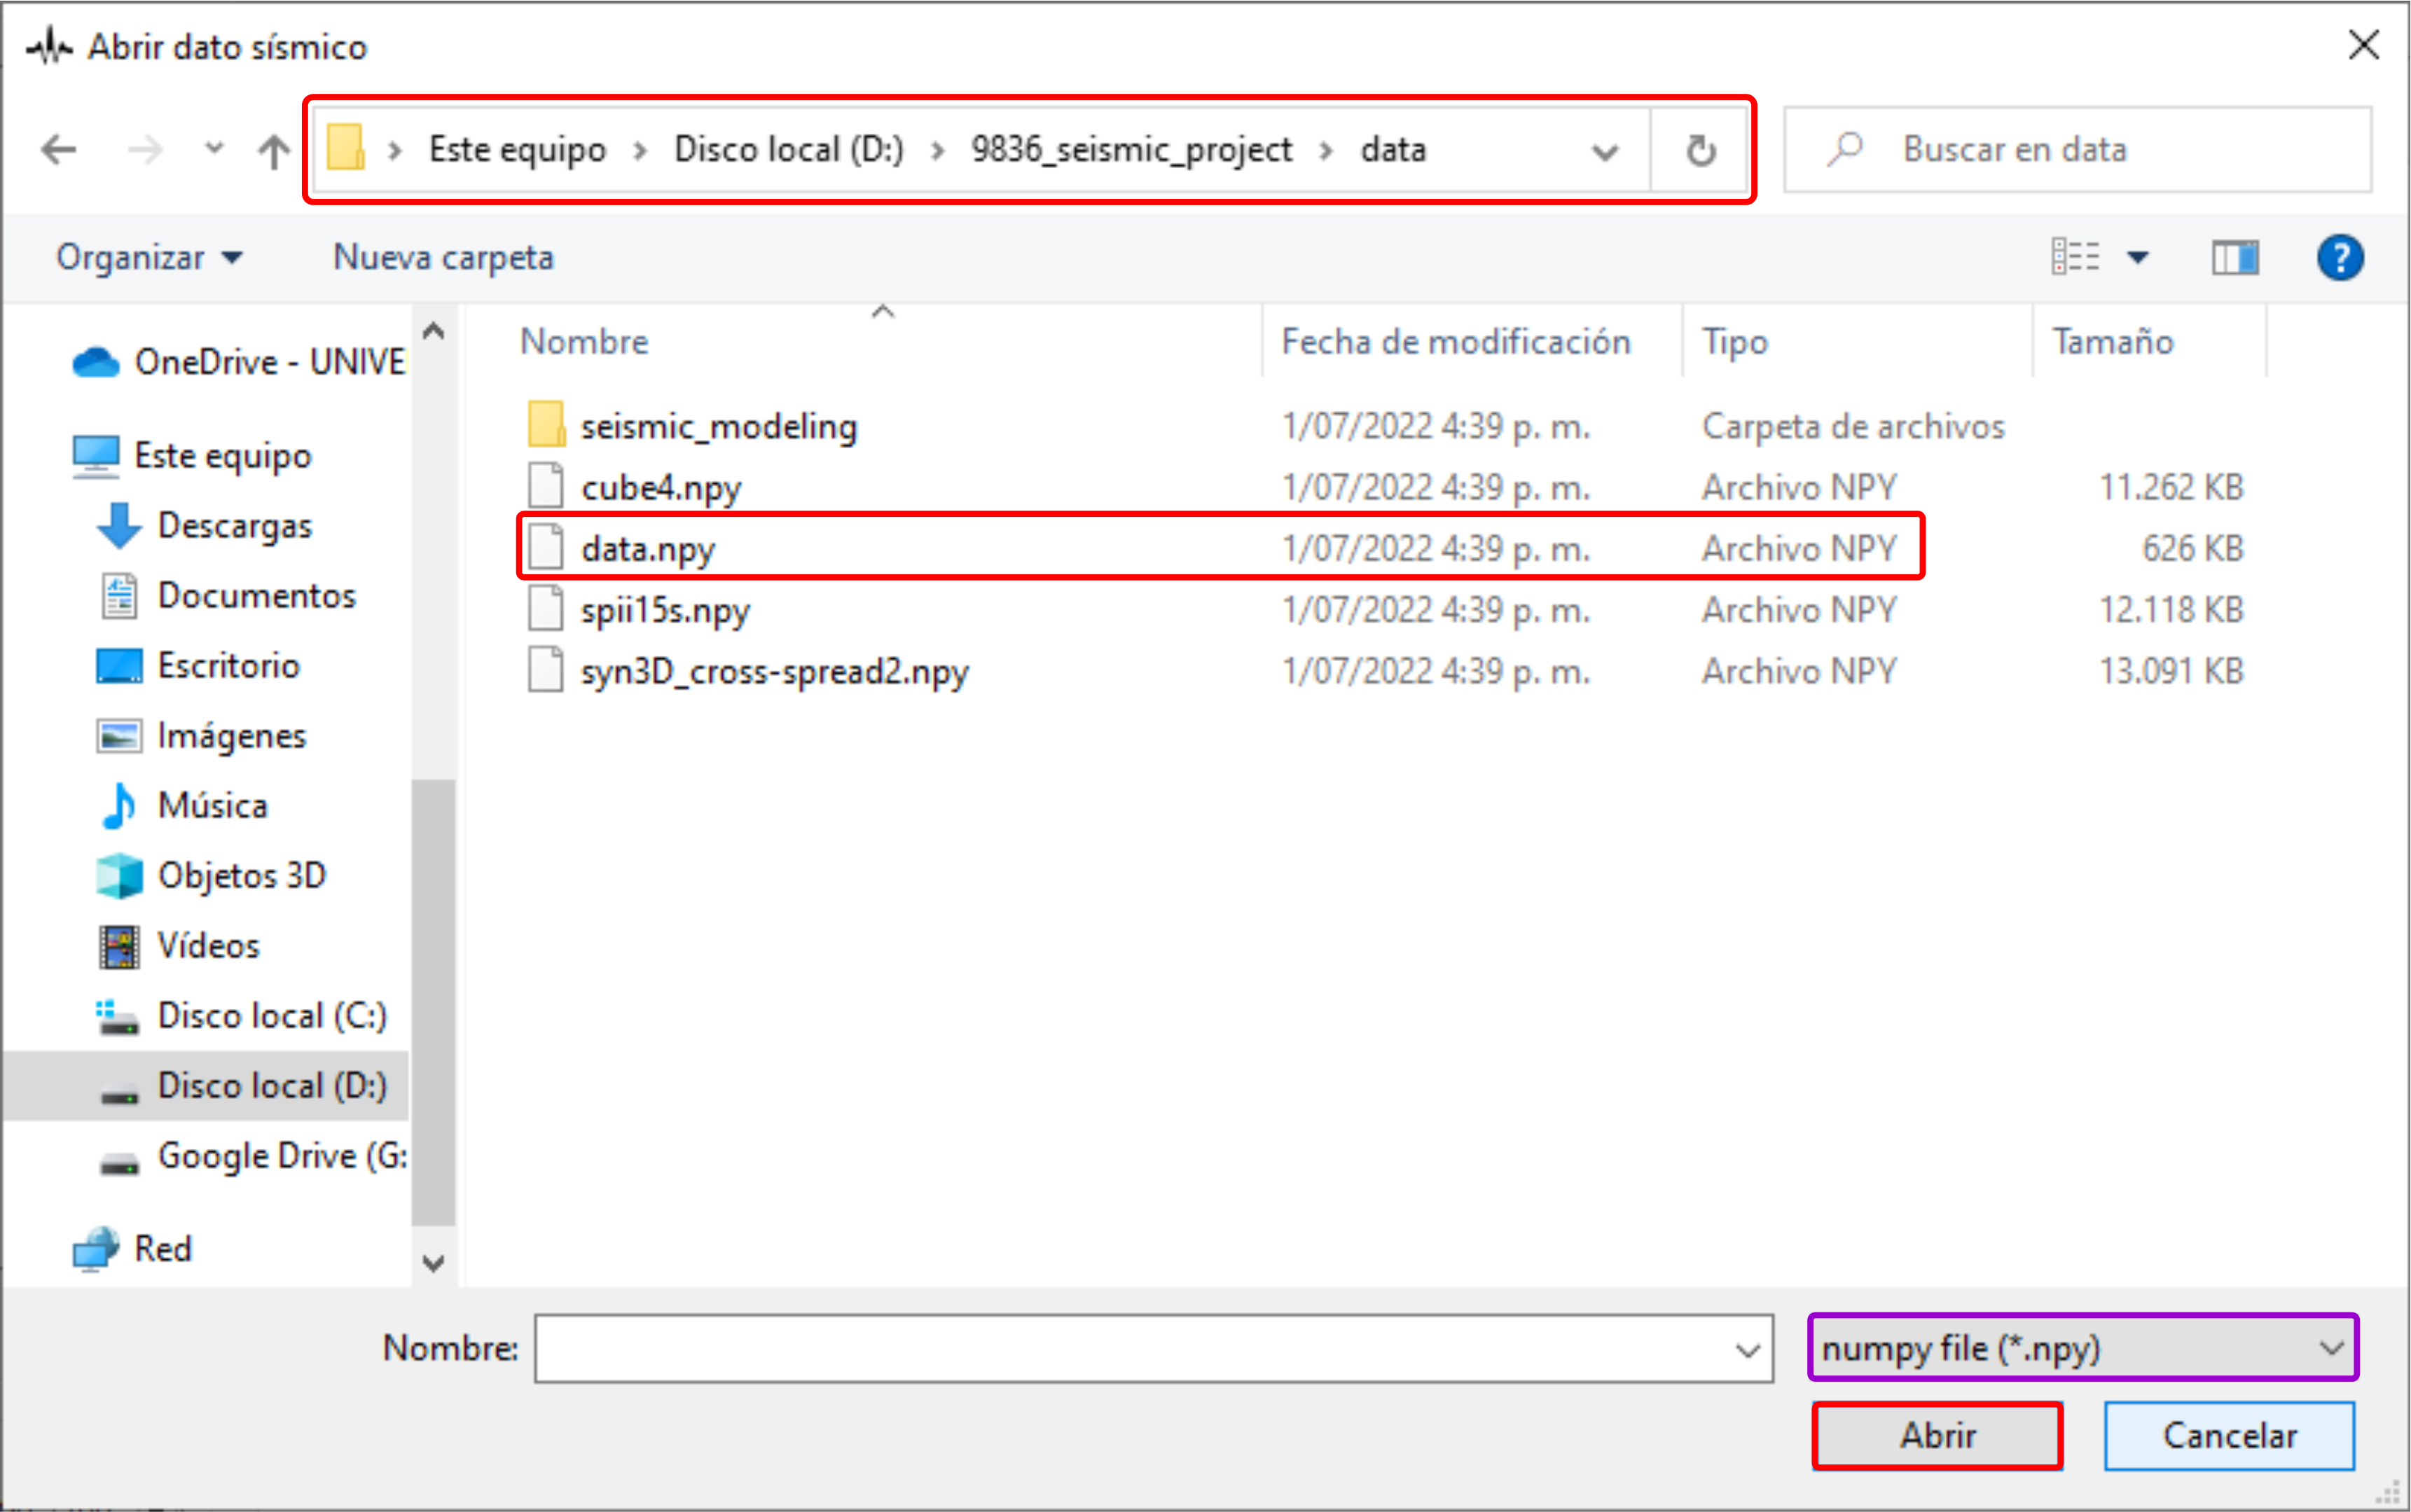
\includegraphics[width=1\linewidth]{data-lecture-2.png}
     \captionof{figure}{Ventana de selección de dato sísmico.}
    \label{fig:data_lecture_2}
\end{Figure}

Existen dos tipos de datos sísmicos que pueden ser cargados desde ReDs: \textit{Datos Completos} y \textit{Datos Incompletos}. El tipo de dato a ser cargado puede ser seleccionado desde la lista desplegable en la Figura \ref{fig:data_lecture_1}.

\begin{multicols}{2}

Una vez seleccionado el dato sísmico, se debe pulsar en la opción \emph{Abrir}. Se podrá observar entonces en \circled{2} el dato sísmico cargado, como se muestra en la figura \ref{fig:data_lecture_3}. Aquí los datos se observan siguiendo la siguiente estructura: \circled{I} representa al directorio padre y \circled{II} es el dato sísmico cargado hijo del directorio padre.

\begin{Figure}
    \centering
    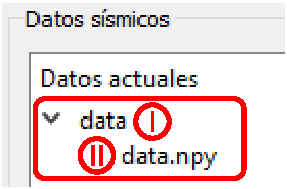
\includegraphics[width=0.6\linewidth]{data-lecture-3.pdf}
     \captionof{figure}{Panel con un dato sísmico cargado.}
    \label{fig:data_lecture_3}
\end{Figure}

\end{multicols}

\subsubsection{Algoritmos}

Los algoritmos disponibles en la aplicación son \emph{FISTA}, \emph{GAP}, \emph{TwIST} y \emph{ADMM}, tal como se observa en el panel \circled{3}, en el extremo izquierdo de la figura \ref{fig:vision}. En este panel se pueden observar las opciones de configuración de parámetros según el algoritmo seleccionado, incluyendo la cantidad máxima de iteraciones a realizar. 

\begin{figure}[!ht]
     \centering
     \begin{subfigure}[b]{0.47\textwidth}
         \centering
         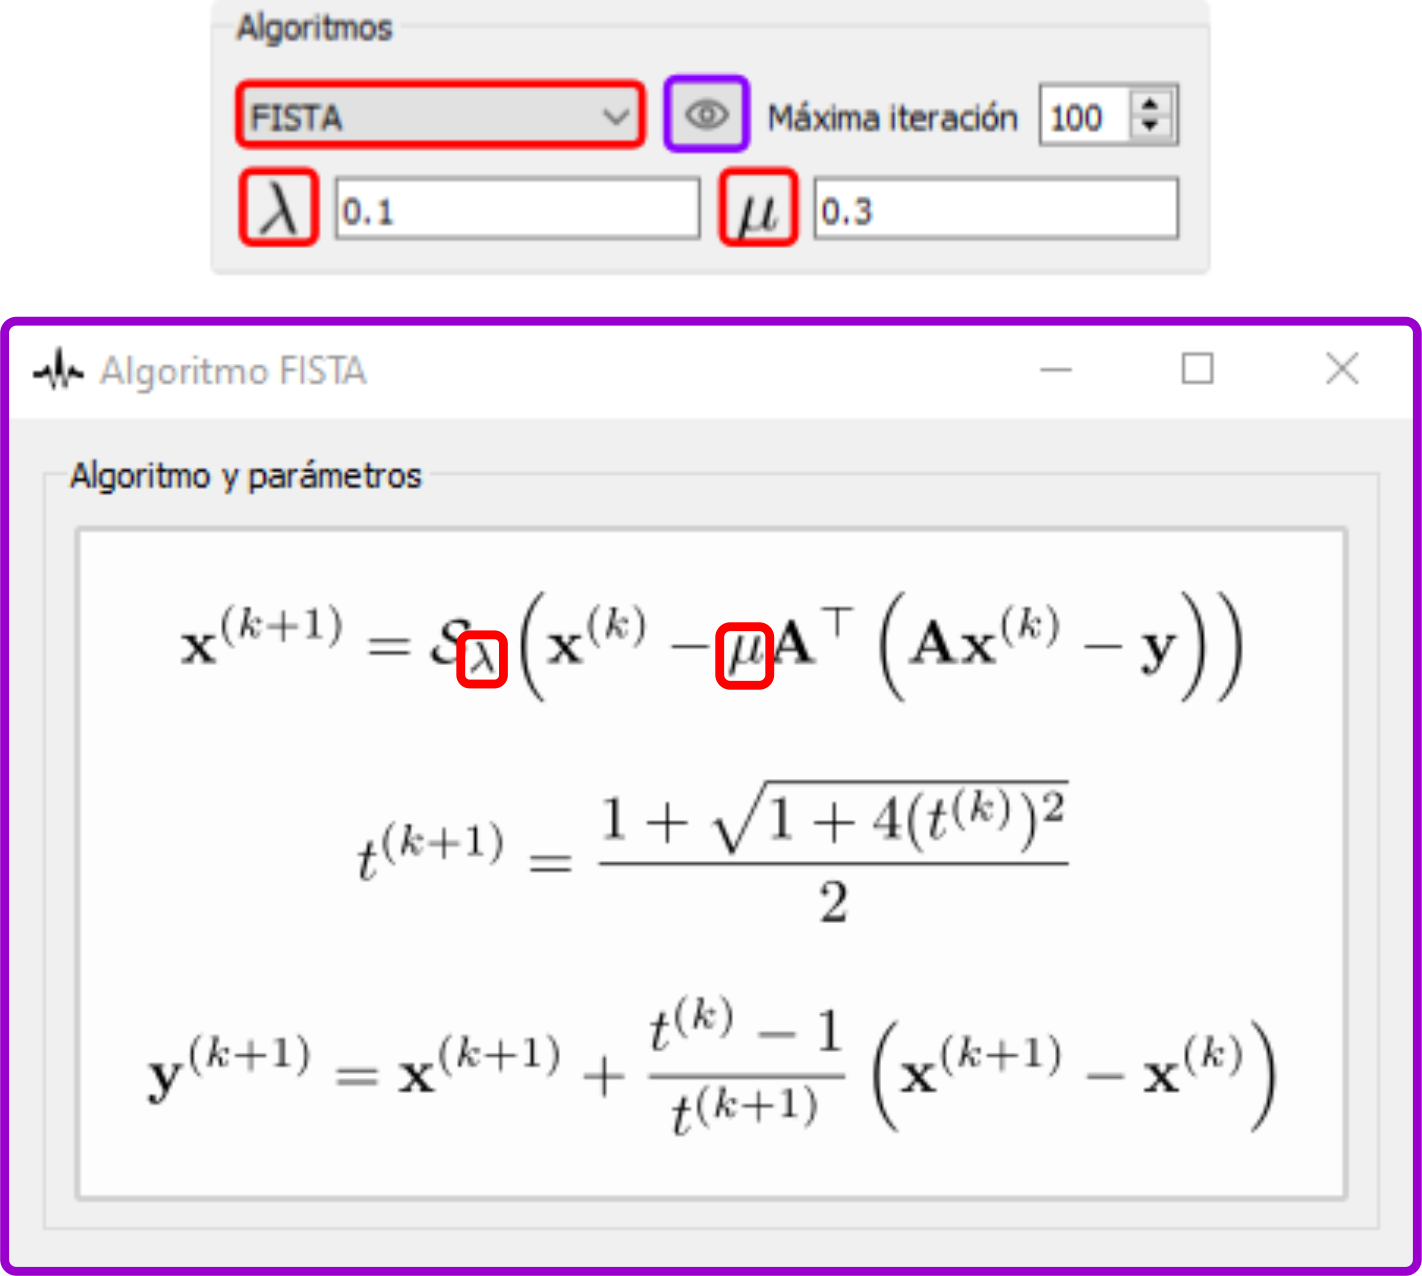
\includegraphics[width=\textwidth]{algorithm-fista.png}
         \caption{FISTA}
         \label{fig:fista}
     \end{subfigure}
     \hfill
     \begin{subfigure}[b]{0.47\textwidth}
         \centering
         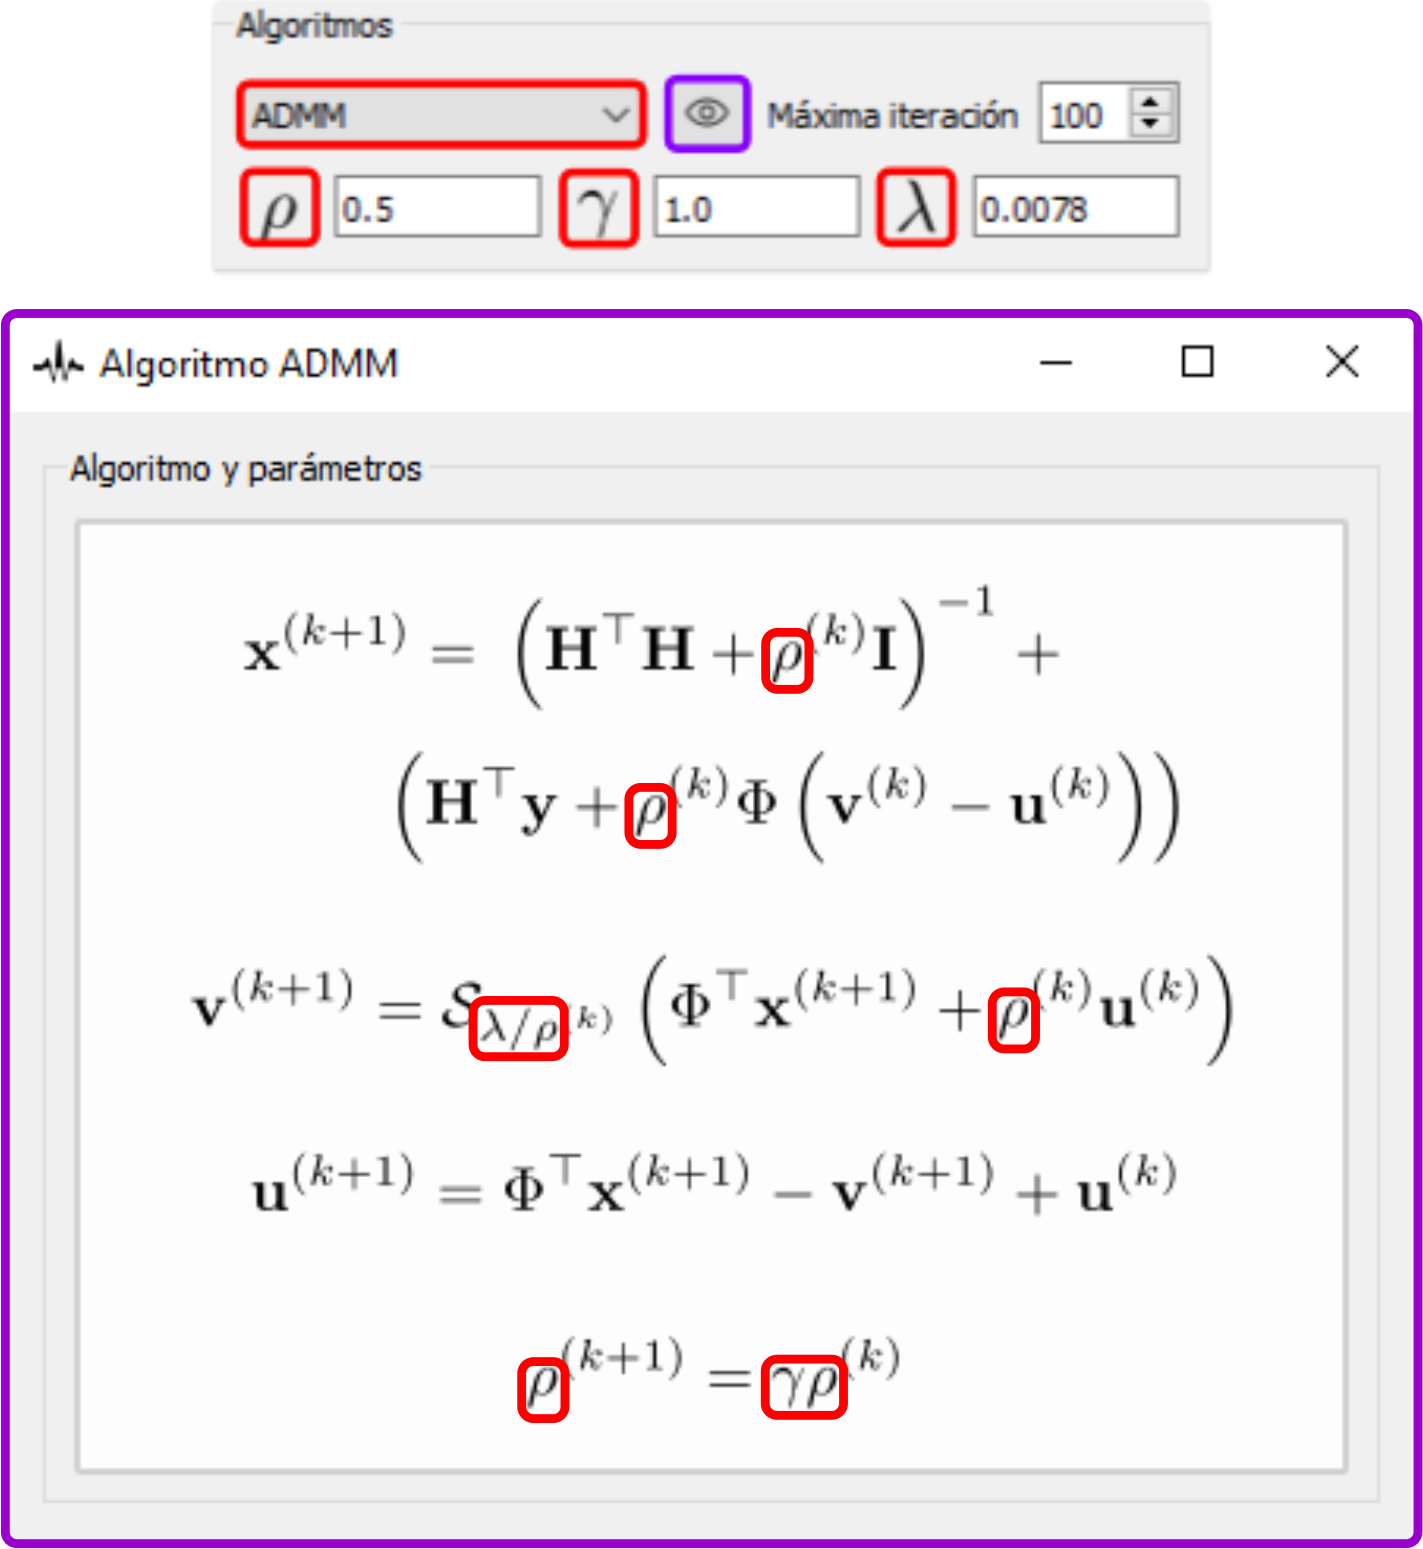
\includegraphics[width=\textwidth]{algorithm-admm.png}
         \caption{ADMM}
         \label{fig:admm}
     \end{subfigure}
     \begin{subfigure}[b]{0.47\textwidth}
         \centering
         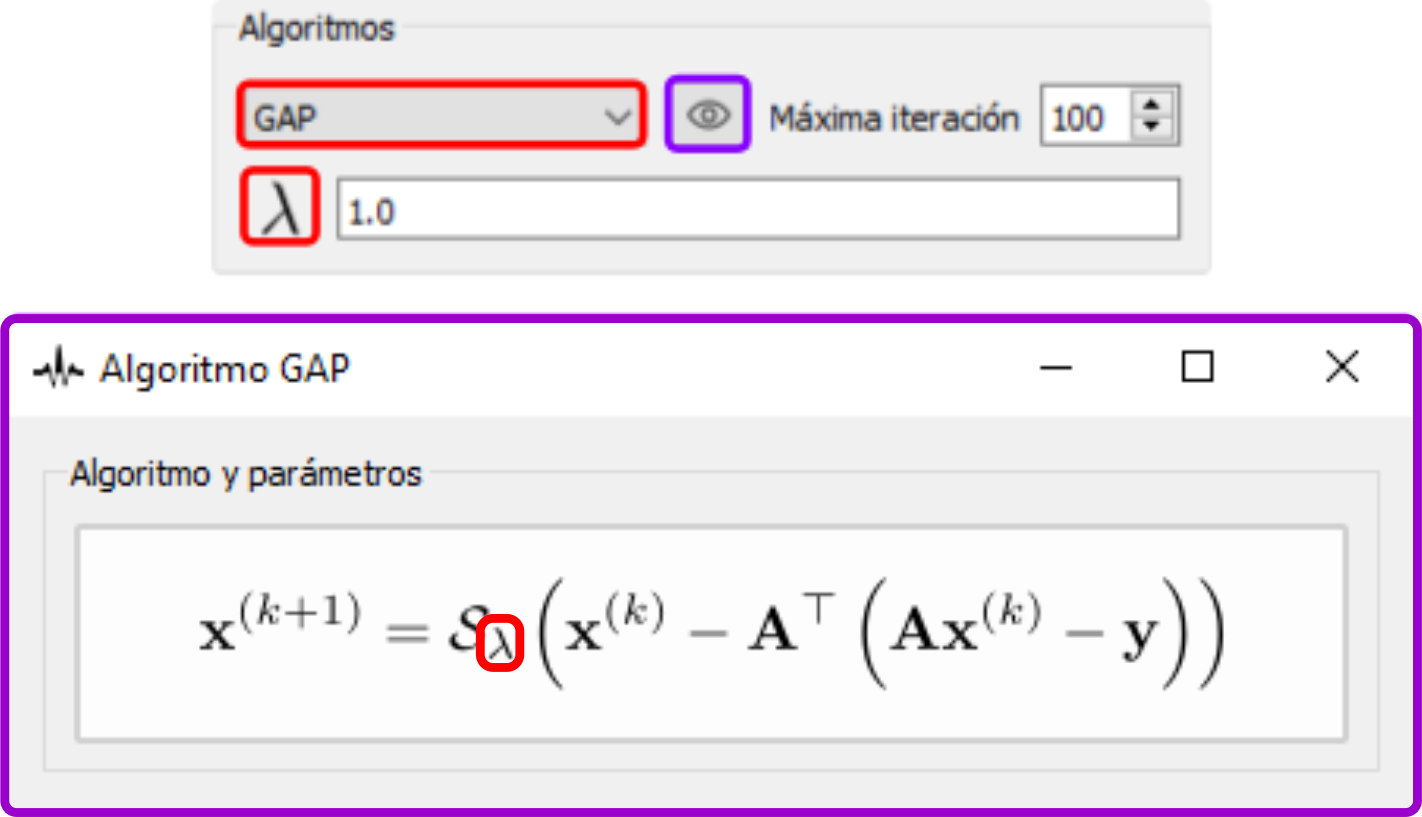
\includegraphics[width=\textwidth]{algorithm-gap.png}
         \caption{GAP}
         \label{fig:gap}
     \end{subfigure}
     \hfill
     \begin{subfigure}[b]{0.47\textwidth}
         \centering
         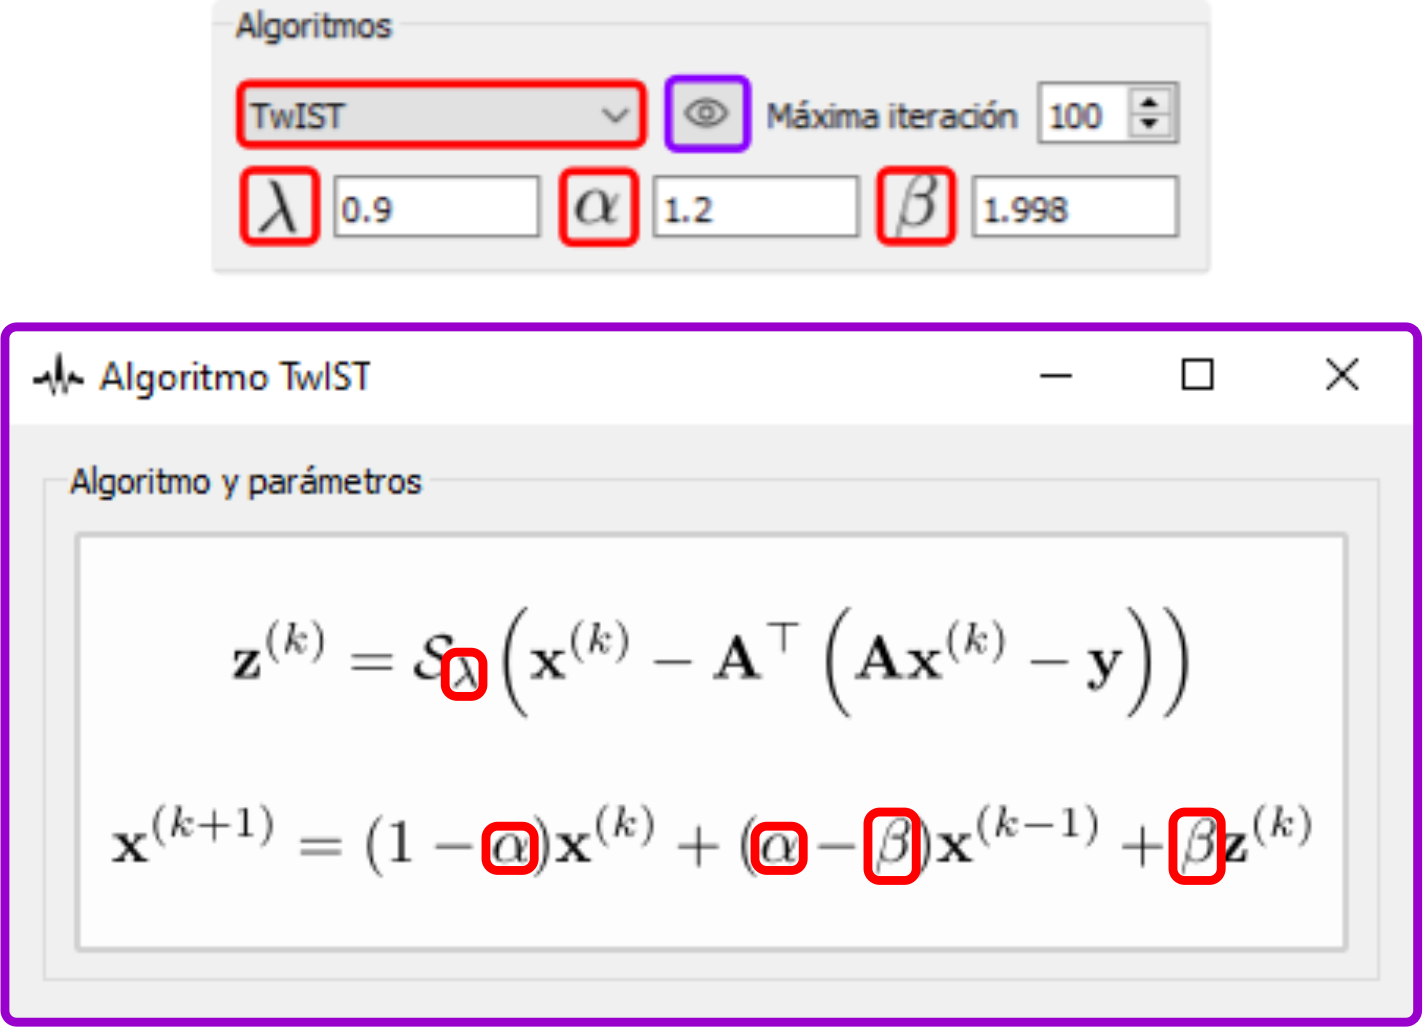
\includegraphics[width=\textwidth]{algorithm-twist.png}
         \caption{TwIST}
         \label{fig:twist}
     \end{subfigure}
        \caption{Algoritmos disponibles y sus respectivos parámetros.}
        \label{fig:algorithms}
\end{figure}

Adicionalmente, el botón\hspace{0.5mm} \faEye \hspace{0.5mm} permite visualizar los diferentes algoritmos con sus correspondientes parámetros, como se observa en la figura \ref{fig:algorithms}. Cada uno de los algoritmos disponibles cuenta con una colección propia de parámetros, los cuales el pueden ser configurados por el usuario según lo desee.

\subsubsection{Submuestreo}\label{subsampling}

Debido a que hay varias formas de recuperar una traza a partir de las medidas recolectadas previamente, el panel de submuestreo \circled{4} permite configurar cuál tipo de submuestreo se desea realizar al dato sísmico, a manera de simulación. Todos los tipos de submuestreo, excepto el de tipo lista, comparten el mismo nivel de compresión que el usuario desee asignar. A continuación se presentan los tipos de submuestreo a aplicar en ReDs:\\

\underline{\textbf{Submuestreo Aleatorio}}

\begin{multicols}{2}
\begin{Figure}
	\centering
	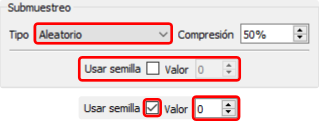
\includegraphics[width=0.8\linewidth]{subsampling-random.png}
	\captionof{figure}{Submuestreo aleatorio.}
	\label{fig:subsampling_random}
\end{Figure}

Aplica un submuestreo aleatorio a las trazas sísmicas de acuerdo al nivel de compresión. Al habilitar la semilla, se puede establecer el mismo submuestreo para todas las veces que se ejecute un experimento, como se observa en la figura \ref{fig:subsampling_random}.

\end{multicols}

\underline{\textbf{Submuestreo Uniforme}}

\begin{multicols}{2}

Aplica un submuestreo uniforme a las trazas sísmicas de acuerdo al nivel de compresión, como se observa en la figura \ref{fig:subsampling_uniform}.

\begin{Figure}
    \centering
    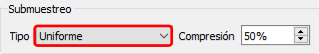
\includegraphics[width=0.8\linewidth]{subsampling-uniform.png}
     \captionof{figure}{Submuestreo uniforme.}
    \label{fig:subsampling_uniform}
\end{Figure}

\end{multicols}

\underline{\textbf{Submuestreo Jitter}}

\begin{multicols}{2}

\begin{Figure}
	\centering
	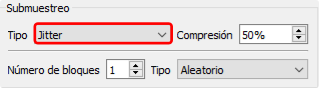
\includegraphics[width=0.8\linewidth]{subsampling-jitter.png}
	\captionof{figure}{Submuestreo jitter.}
	\label{fig:subsampling_jitter}
\end{Figure}

Aplica un submuestreo aleatorio o uniforme de acuerdo a la cantidad de bloques ingresados por el usuario a las trazas sísmicas de acuerdo al nivel de compresión, como se observa en la figura \ref{fig:subsampling_jitter}.

\end{multicols}

\underline{\textbf{Submuestreo Lista}}

\begin{multicols}{2}

Aplica un submuestreo de tipo lista donde las trazas a remover son ingresados por el usuario, como se observa en la figura \ref{fig:subsampling_list}. Para este tipo de submuestreo es necesario validar que el usuario ingrese los datos con un formato lógico y especifico.

\begin{Figure}
    \vspace{5mm}
    \centering
    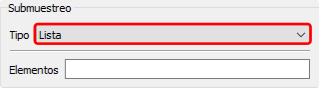
\includegraphics[width=0.8\linewidth]{subsampling-list.png}
     \captionof{figure}{Submuestreo de tipo lista.}
    \label{fig:subsampling_list}
\end{Figure}

\end{multicols}

Las condiciones son las siguientes:

\begin{multicols}{2}

\begin{Figure}
	\vspace{5mm}
	\centering
	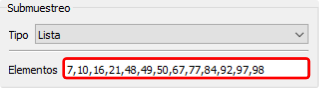
\includegraphics[width=1\linewidth]{subsampling-list-1.png}
	\captionof{figure}{Ejemplo de submuestreo de tipo lista.}
	\label{fig:subsampling_list_1}
\end{Figure}

\begin{itemize}
	\setlength\itemsep{0em}
    \item La secuencia debe ser $x_1,x_2,x_n$, tal que $x_i \in \mathbb{Z}^+$ representa los índices de las trazas a resolver, donde entre cada $x_i$ no deben haber espacios y estar separados por números, como se observa en la figura \ref{fig:subsampling_list_1}.
    \item Cada $x_i$ debe cumplir $0 \leq x_i \leq N$, donde $N$ es la cantidad máxima lineas de receptores que contiene un \emph{shot}.
    \item Deben haber mínimo siete $x_i$ distintos.
\end{itemize}

\end{multicols}

\subsubsection{Experimentos}
\label{sec:experiment}

Una vez ya se ha cargado un dato sísmico, seleccionado el algoritmo, ajustado sus parámetros y configurado el tipo de submuestreo, entonces se podrá realizar un experimento. El panel \circled{5}, en el extremo izquierdo de la figura \ref{fig:vision}, permite controlar el progreso de la ejecución del experimento a realizar.

\subsubsection*{Realizando un experimento}

\begin{multicols}{2}

Para iniciar un nuevo experimento se debe pulsar el botón \hspace{0.5mm} \faSave \hspace{0.5mm} que se observa en la figura \ref{fig:experiment_1}. Aquí el usuario seleccionará el directorio donde desee que los resultados de su experimento sean guardados, como se observa en la figura \ref{fig:experiment_2}.

\begin{Figure}
    \vspace{5mm}
    \centering
    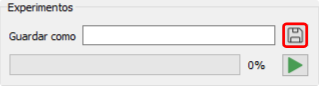
\includegraphics[width=0.8\linewidth]{experiment-1.png}
     \captionof{figure}{Panel de experimentos.}
    \label{fig:experiment_1}
\end{Figure}

\end{multicols}

\begin{Figure}
    \centering
    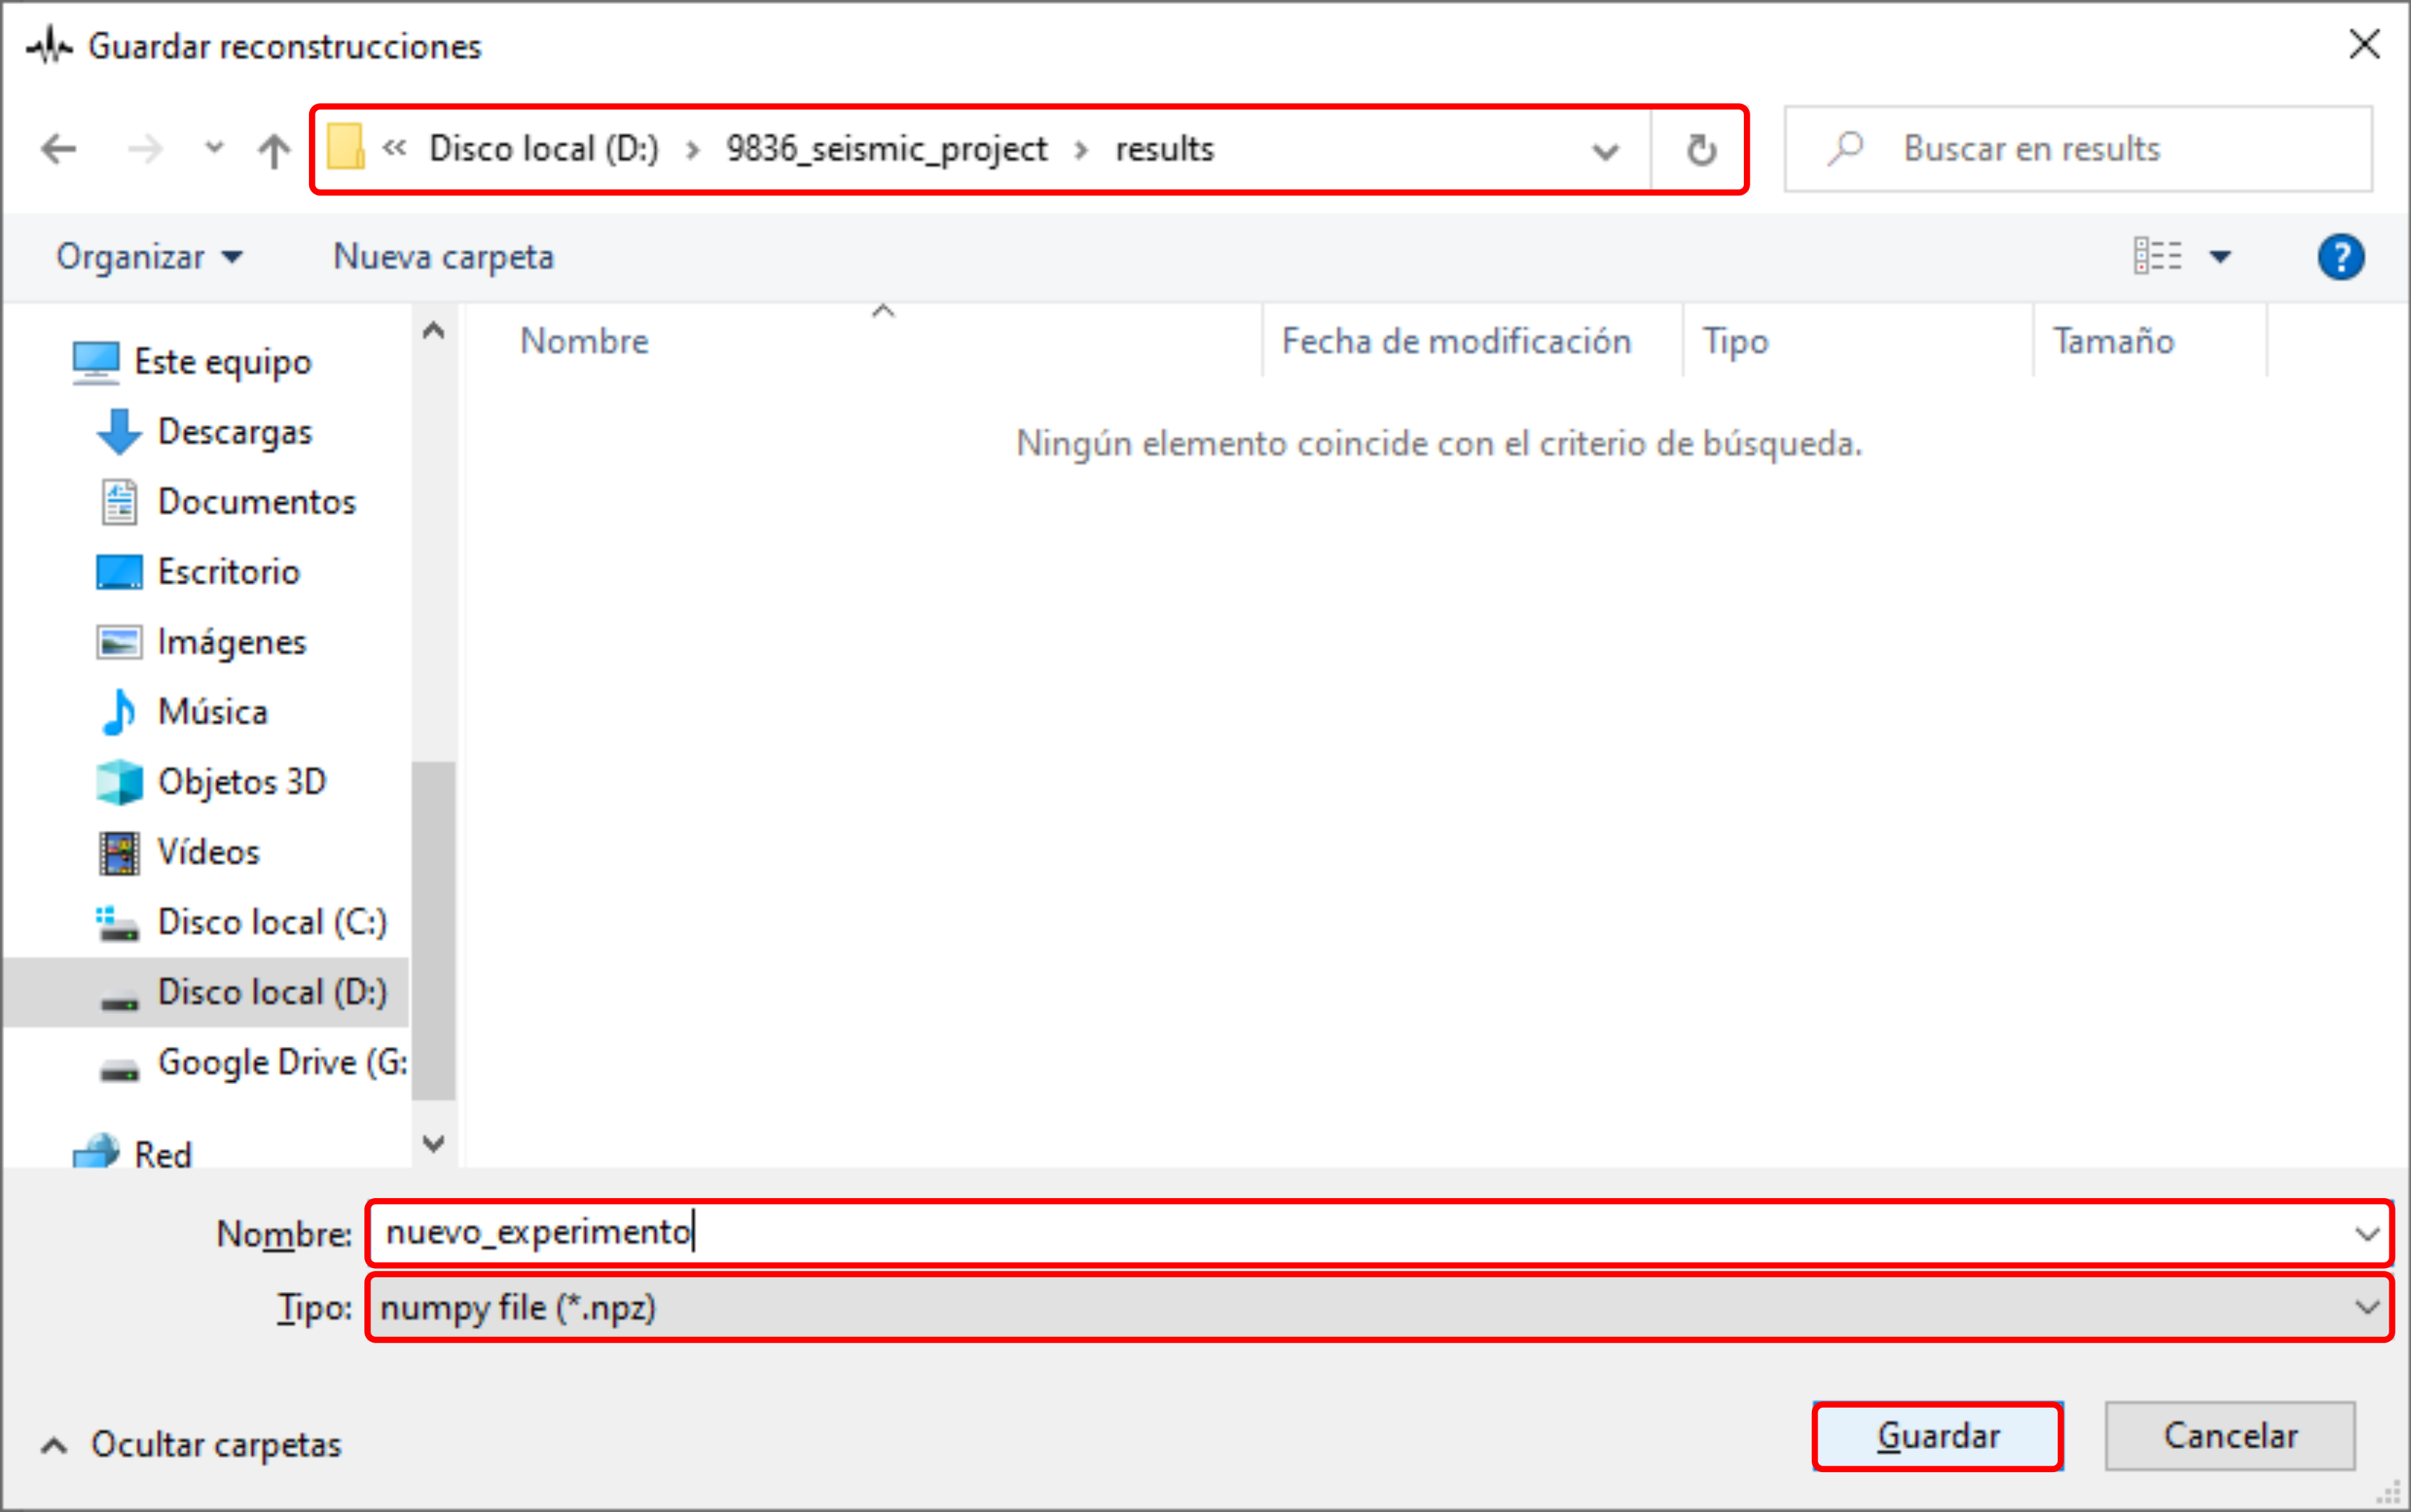
\includegraphics[width=1\linewidth]{experiment-2.png}
     \captionof{figure}{Ventana de guardado de resultados.}
    \label{fig:experiment_2}
\end{Figure}

Es necesario asignar un nombre al experimento para poder guardarlo. En este ejemplo usaremos \emph{nuevo\_experimento} como nombre del archivo de salida, con la extensión \emph{.npz}. Finalmente, presionamos el botón \emph{Guardar}.

\begin{multicols}{2}

\begin{Figure}
	\centering
	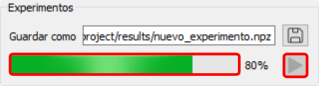
\includegraphics[width=0.7\linewidth]{experiment-4.png}
	\captionof{figure}{Ejecución de un experimento en tiempo real.}
	\label{fig:experiment_4}
\end{Figure}

Para correr el experimento se debe pulsar en el botón \hspace{0.5mm} \faPlay \hspace{0.5mm}. En la barra de progreso, a la izquierda de dicho botón, se podrá el progreso del actual experimento, como se observa en la figura \ref{fig:experiment_4}.

\end{multicols}

\subsubsection{Visualización de Resultados}

Finalmente, los resultados de todos los experimentos que se realicen a través de esta aplicación se pueden observar en el panel \circled{7}, en el extremo derecho de la figura \ref{fig:vision}. En este panel se encuentran dos tipos de visualización: la visualización del rendimiento (iteraciones vs. error/psnr) y visualización de la reconstrucción, como se observa en la figura \ref{fig:main_result_1}.

\begin{multicols}{2}

Como se mencionó en la sección \ref{sec:experiment}, para los experimentos que sean ejecutados se podrá ver tanto el rendimiento como la reconstrucción de las trazas en tiempo real. A continuación se detallará que es lo que se observa exactamente en cada una de estos subpaneles.

\begin{Figure}
    %\vspace{1cm}
    \centering
    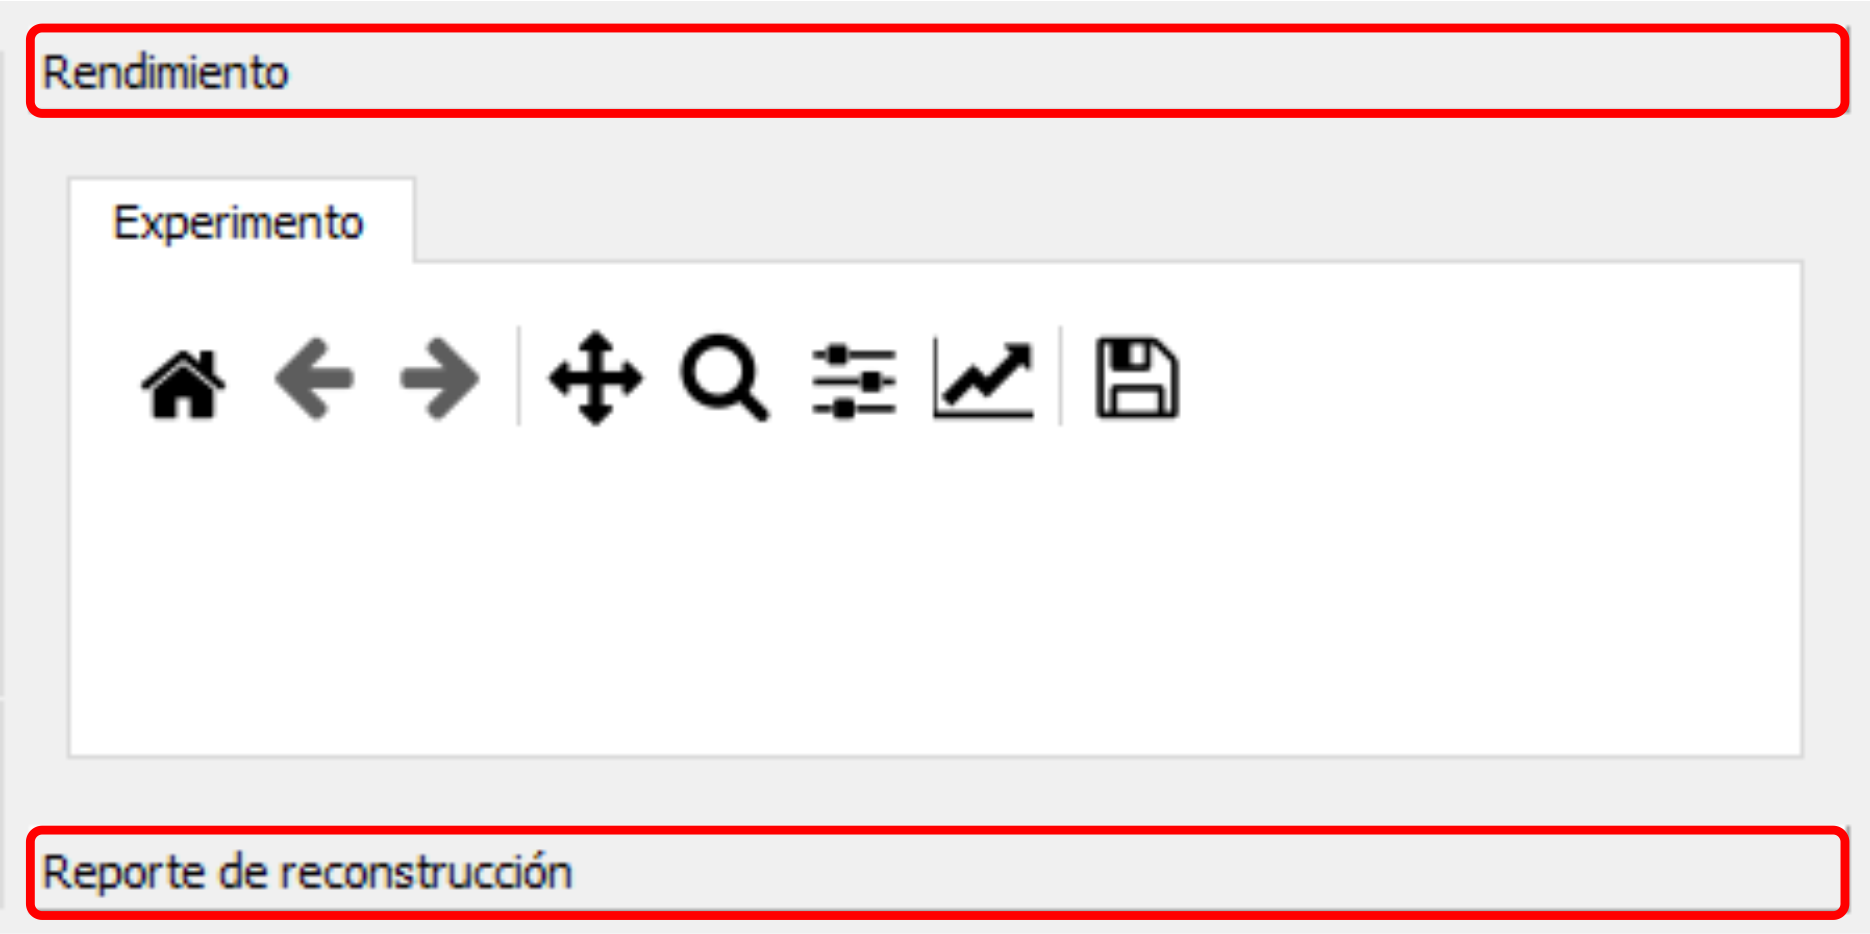
\includegraphics[width=0.7\linewidth]{main-result-1.png}
     \captionof{figure}{Panel de resultados.}
    \label{fig:main_result_1}
\end{Figure}

\end{multicols}

\subsubsection*{Rendimiento}

En esta subventana se observa el rendimiento actual del experimento que esté corriendo, como se muestra en la figura \ref{fig:main_result_2}. Esta figura presenta una gráfica con dos ejes: el \textcolor{red}{eje izquierdo} representa el indice de similaridad estructural (SSIM); y el \textcolor{blue}{eje derecho} representa la proporción máxima de señal a ruido (PSNR) de las trazas reconstruidas con respecto a las verdaderas. En general, ambas métricas cuantifican la degradación de la calidad de la imagen.

\begin{Figure}
	\centering
	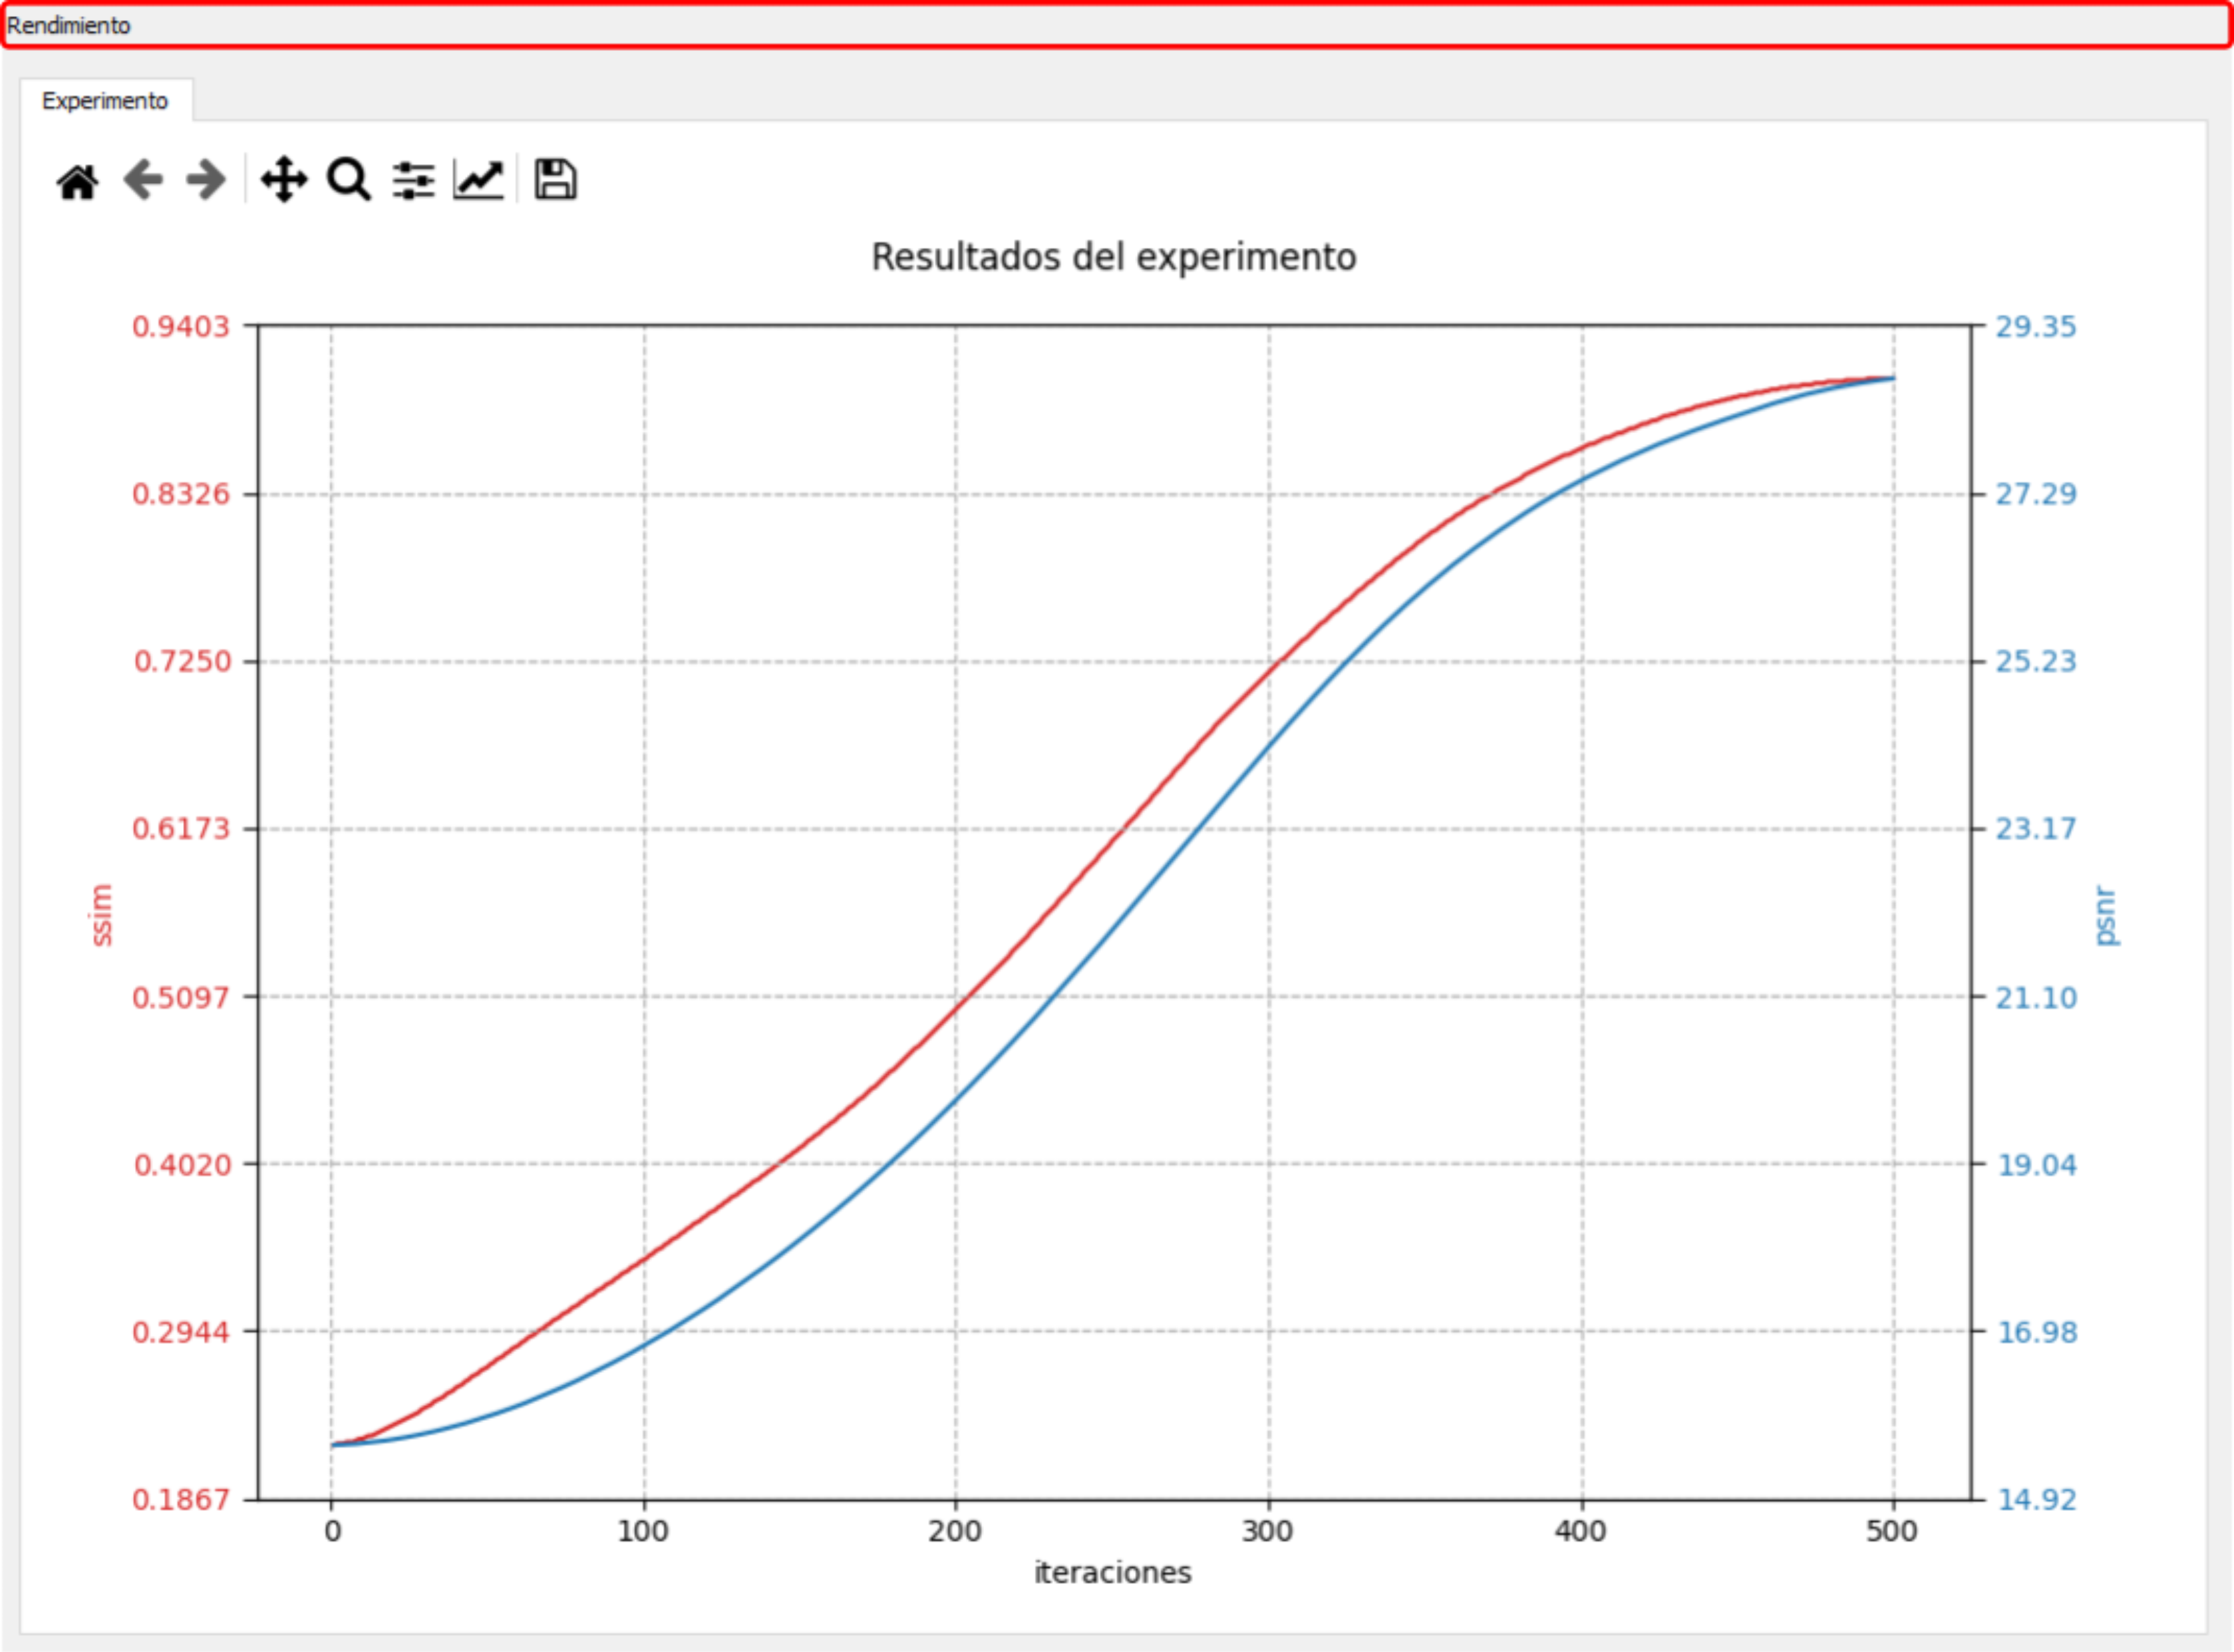
\includegraphics[width=0.8\linewidth]{main-result-2.png}
	\captionof{figure}{Rendimiento de un experimento realizado.}
	\label{fig:main_result_2}
\end{Figure}

\begin{multicols}{2}

\begin{Figure}
	\vspace{0.7cm}
	\centering
	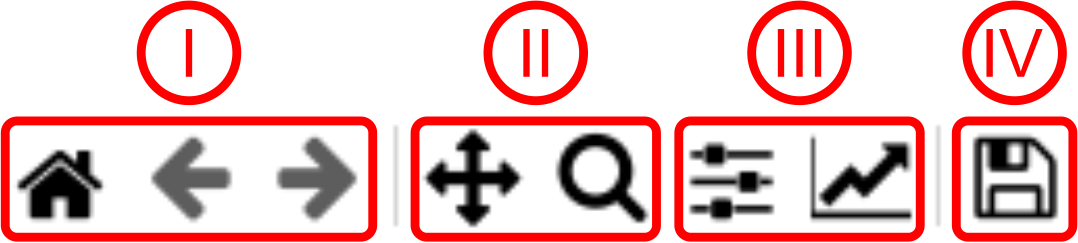
\includegraphics[width=0.9\linewidth]{main-result-3.png}
	\captionof{figure}{Opciones de la gráfica.}
	\label{fig:main_result_3}
\end{Figure}

En la parte superior de la gráfica \textit{Resultados del experimento} se observa una barra de herramientas, tal como se muestra en la figura \ref{fig:main_result_3}. Estas modifican alguna característica de la gráfica de resultados, tal como se indica a continuación:

\end{multicols}

\vspace{0.2cm}

\begin{multicols}{2}

\begin{itemize}
	\setlength\itemsep{0em}
    \item[I.]  El botón \hspace{0.5mm} \faHome \hspace{0.5mm} permite volver a la gráfica a su estado original. Los otros dos botones, \hspace{0.5mm} \faArrowLeft \hspace{0.5mm} y \hspace{0.5mm} \faArrowRight \hspace{0.5mm}, permiten ir hacia adelante o atrás en las modificaciones realizadas a la gráfica.
    
    \item[II.] El botón \hspace{0.5mm} \faArrows \hspace{0.5mm} permite desplazar la gráfica en cualquier dirección, mientras que el botón \hspace{0.5mm} \faSearch \hspace{0.5mm} permite realizar un acercamiento o alejamiento de la gráfica.

\end{itemize}

\vfill\null
\columnbreak

\begin{Figure}
	%\vspace{-1.5cm}
	\centering
	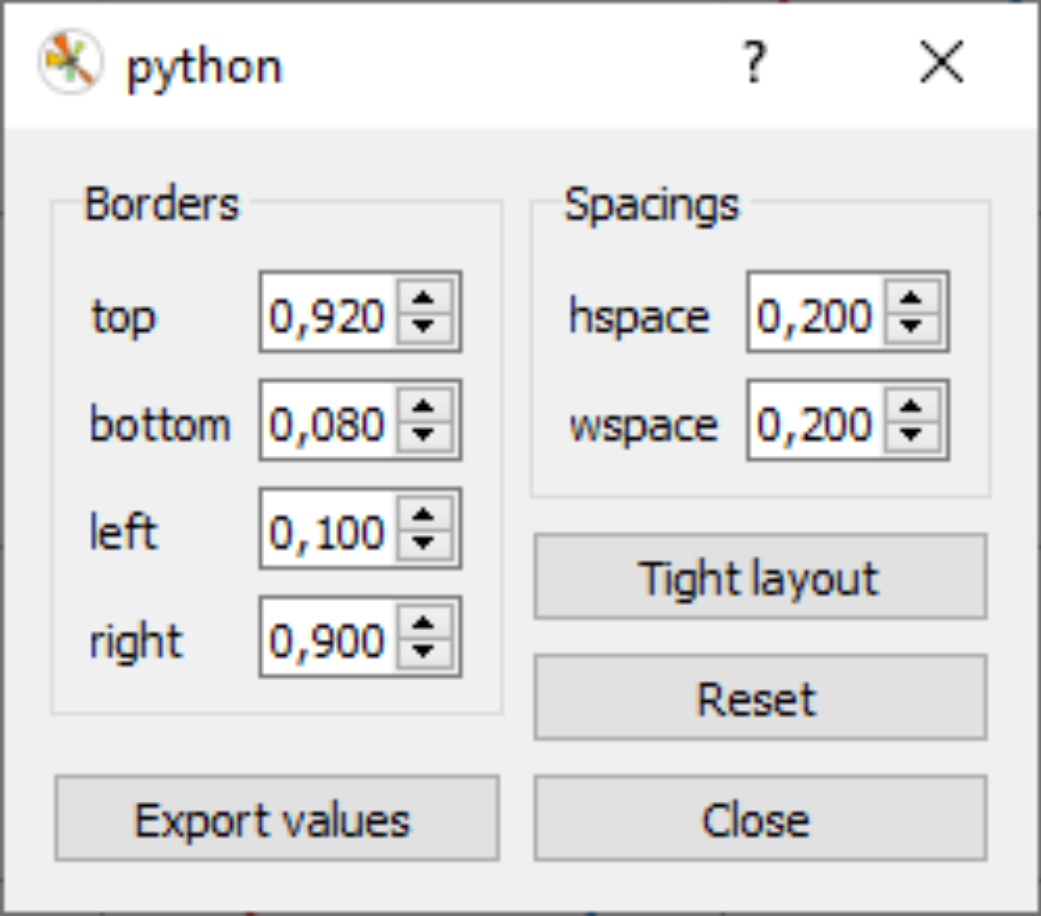
\includegraphics[width=0.6\linewidth]{main-result-4.png}
	\captionof{figure}{Configuración de subplots.}
	\label{fig:main_result_4}
\end{Figure}

\end{multicols}

\begin{multicols}{2}

\begin{Figure}
	%\vspace{-1.5cm}
	\centering
	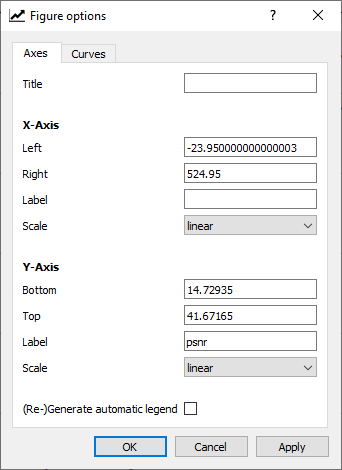
\includegraphics[width=0.7\linewidth]{main-result-5.png}
	\captionof{figure}{Editor de ejes, curvas y parámetros de la gráfica.}
	\label{fig:main_result_5}
\end{Figure}

\vfill\null
\columnbreak

\begin{itemize}
	\setlength\itemsep{0em}
	
	 \item[III.] Los siguientes botones tienen un comportamiento más complejo. El botón \hspace{0.5mm} \faBars \hspace{0.5mm} abre la subventana que se observa en la figura \ref{fig:main_result_4}. Esto permitirá ajustar la visualización de los bordes de la gráfica y el espaciado con respecto a su contenedor padre. Por otra parte, el botón \hspace{0.5mm} \faLineChart \hspace{0.5mm} permitirá configurar la visualización de los ejes (cantidad de valores) y el tipo de escala para cada eje, como se observa en la figura \ref{fig:main_result_5}.
	
	\item[IV.] Finalmente, el botón \hspace{0.5mm} \faSave \hspace{0.5mm} permitirá guardar una imagen de la gráfica exactamente como se observe en ese instante. Los formatos soportados para exportar una gráfica son: \textit{.eps}, \textit{.jpg}, \textit{.pgf}, \textit{.pdf}, \textit{.png}, \textit{.ps}, \textit{.raw}, \textit{.svg}, \textit{.tiff}.
\end{itemize}

\end{multicols}

\subsubsection*{Reconstrucción de Trazas}

Por otra parte, los resultados cuantitativos del experimento se observan en el subpanel de \emph{Reporte}, como se muestra en la figura \ref{fig:main_result_6}. Esta gráfica se divide en 4 secciones:

\begin{itemize}[leftmargin=0.5in]
	\setlength\itemsep{0em}
    \item[I.]  \textit{Referencia}. Esta gráfica es el disparo sísmico completo, el cual se usa como referencia para comparar contra la reconstruida, tanto cuantitativa como cualitativamente.
    
    \item[II.] \textit{Medidas}. Está gráfica es el disparo sísmico submuestreado, y es la que pasa a través de los algoritmos para reconstruir las líneas de receptores faltantes.
    
    \item[III.] \textit{Reconstruido}. Está gráfica contiene el disparo sísmico reconstruida.
    
    \item[IV.] \textit{Traza}. Esta gráfica contiene una de las trazas reconstruidas comparada contra la de referencia.
    
\end{itemize}

\begin{Figure}
    \centering
    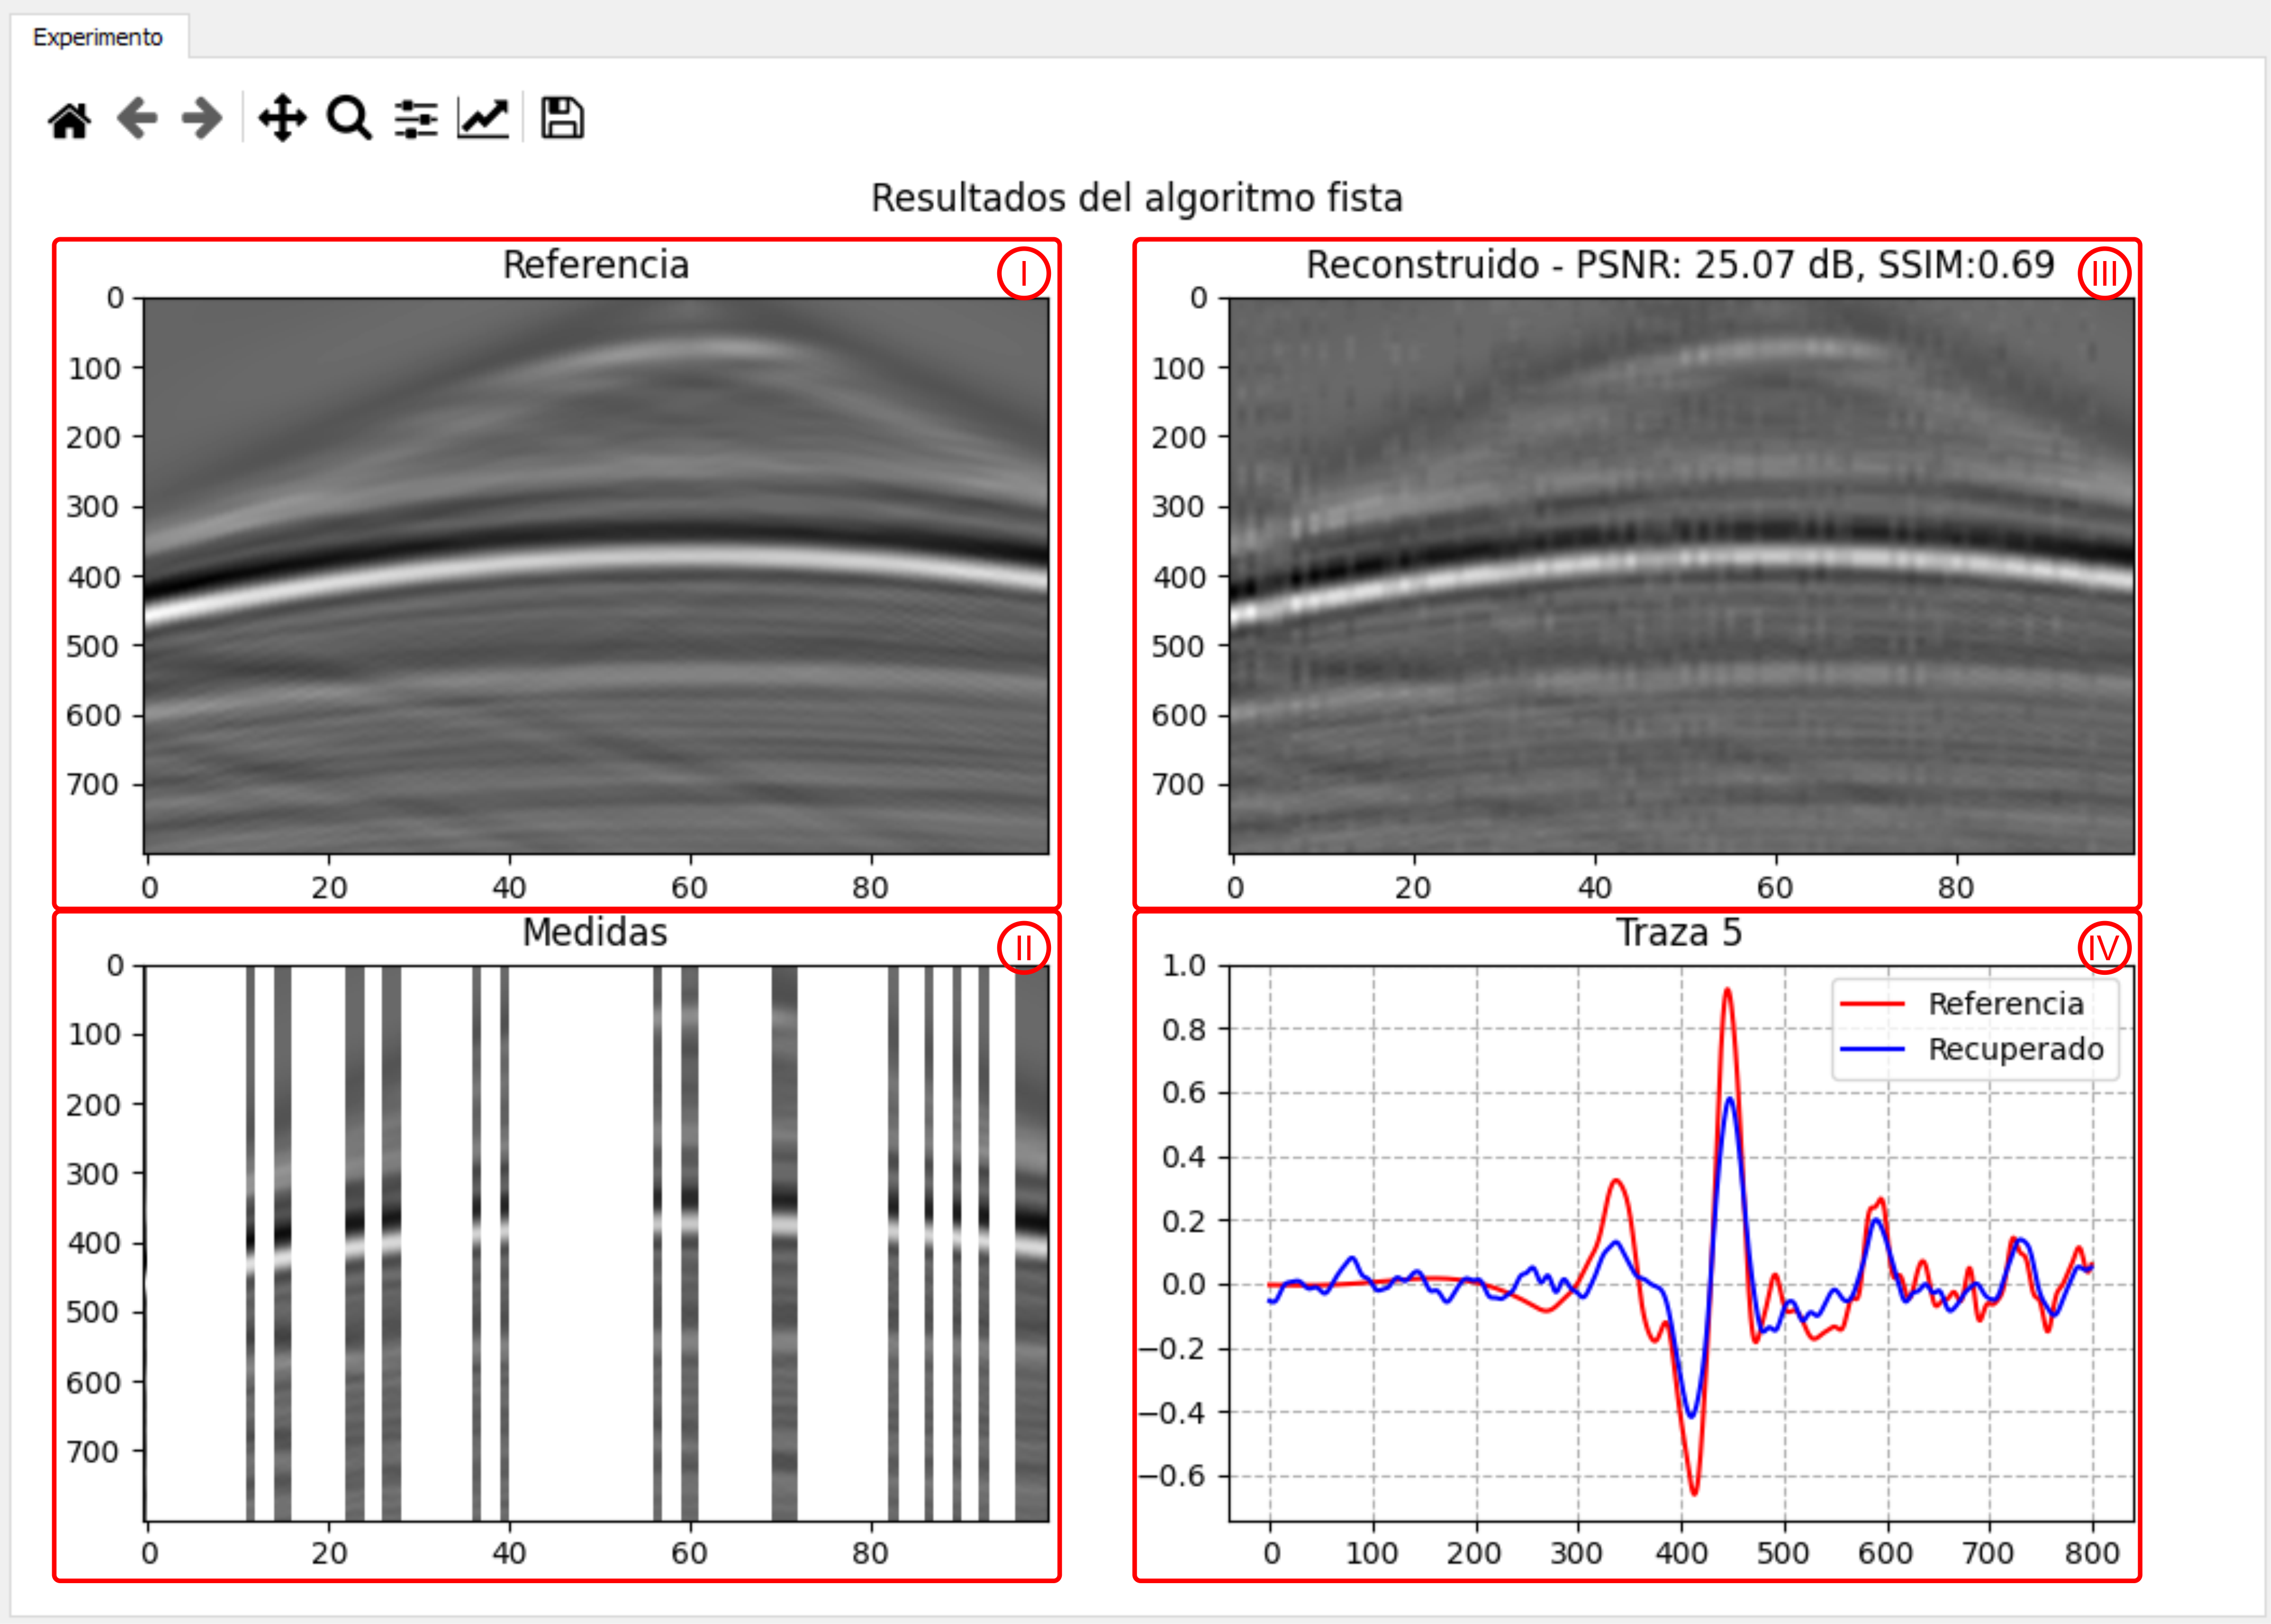
\includegraphics[width=1\linewidth]{main-result-6.png}
     \captionof{figure}{Reporte cuantitativo de un experimento realizado.}
    \label{fig:main_result_6}
\end{Figure}

\vspace{0.5cm}
\subsection{Modo Ajuste de parámetros}

\begin{multicols}{2}

El segundo modo de ejecución de ReDs es el ajuste de parámetros sobre las muestras sísmicas. Este modo se activa usando el segundo botón del menú principal, tal como se muestra en la figura \ref{fig:tuning_button}.

\begin{Figure}
    \centering
    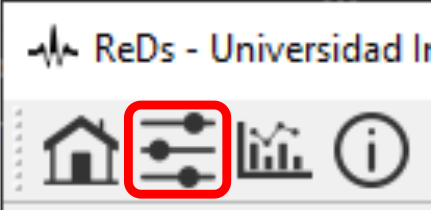
\includegraphics[width=0.4\linewidth]{tuning-tab.png}
     \captionof{figure}{Botón del menú de ajuste de parámetros.}
    \label{fig:tuning_button}
\end{Figure}

\end{multicols}

El ajuste de parámetros permite probar diferentes rangos de parámetros para cada uno de los algoritmos de una forma sencilla y visualizar la curva de rendimiento en dichos ajustes.

La aplicación ReDs se adapta a los tipos de pruebas que se quieran realizar, por lo que la aplicación deshabilita los paneles u opciones que no son necesarias para el ajuste de parámetros, en este caso, y se habilita un nuevo panel llamado \emph{Ajuste de parámetros}, como se observa en la figura \ref{fig:tuning}.

\begin{Figure}
    \centering
    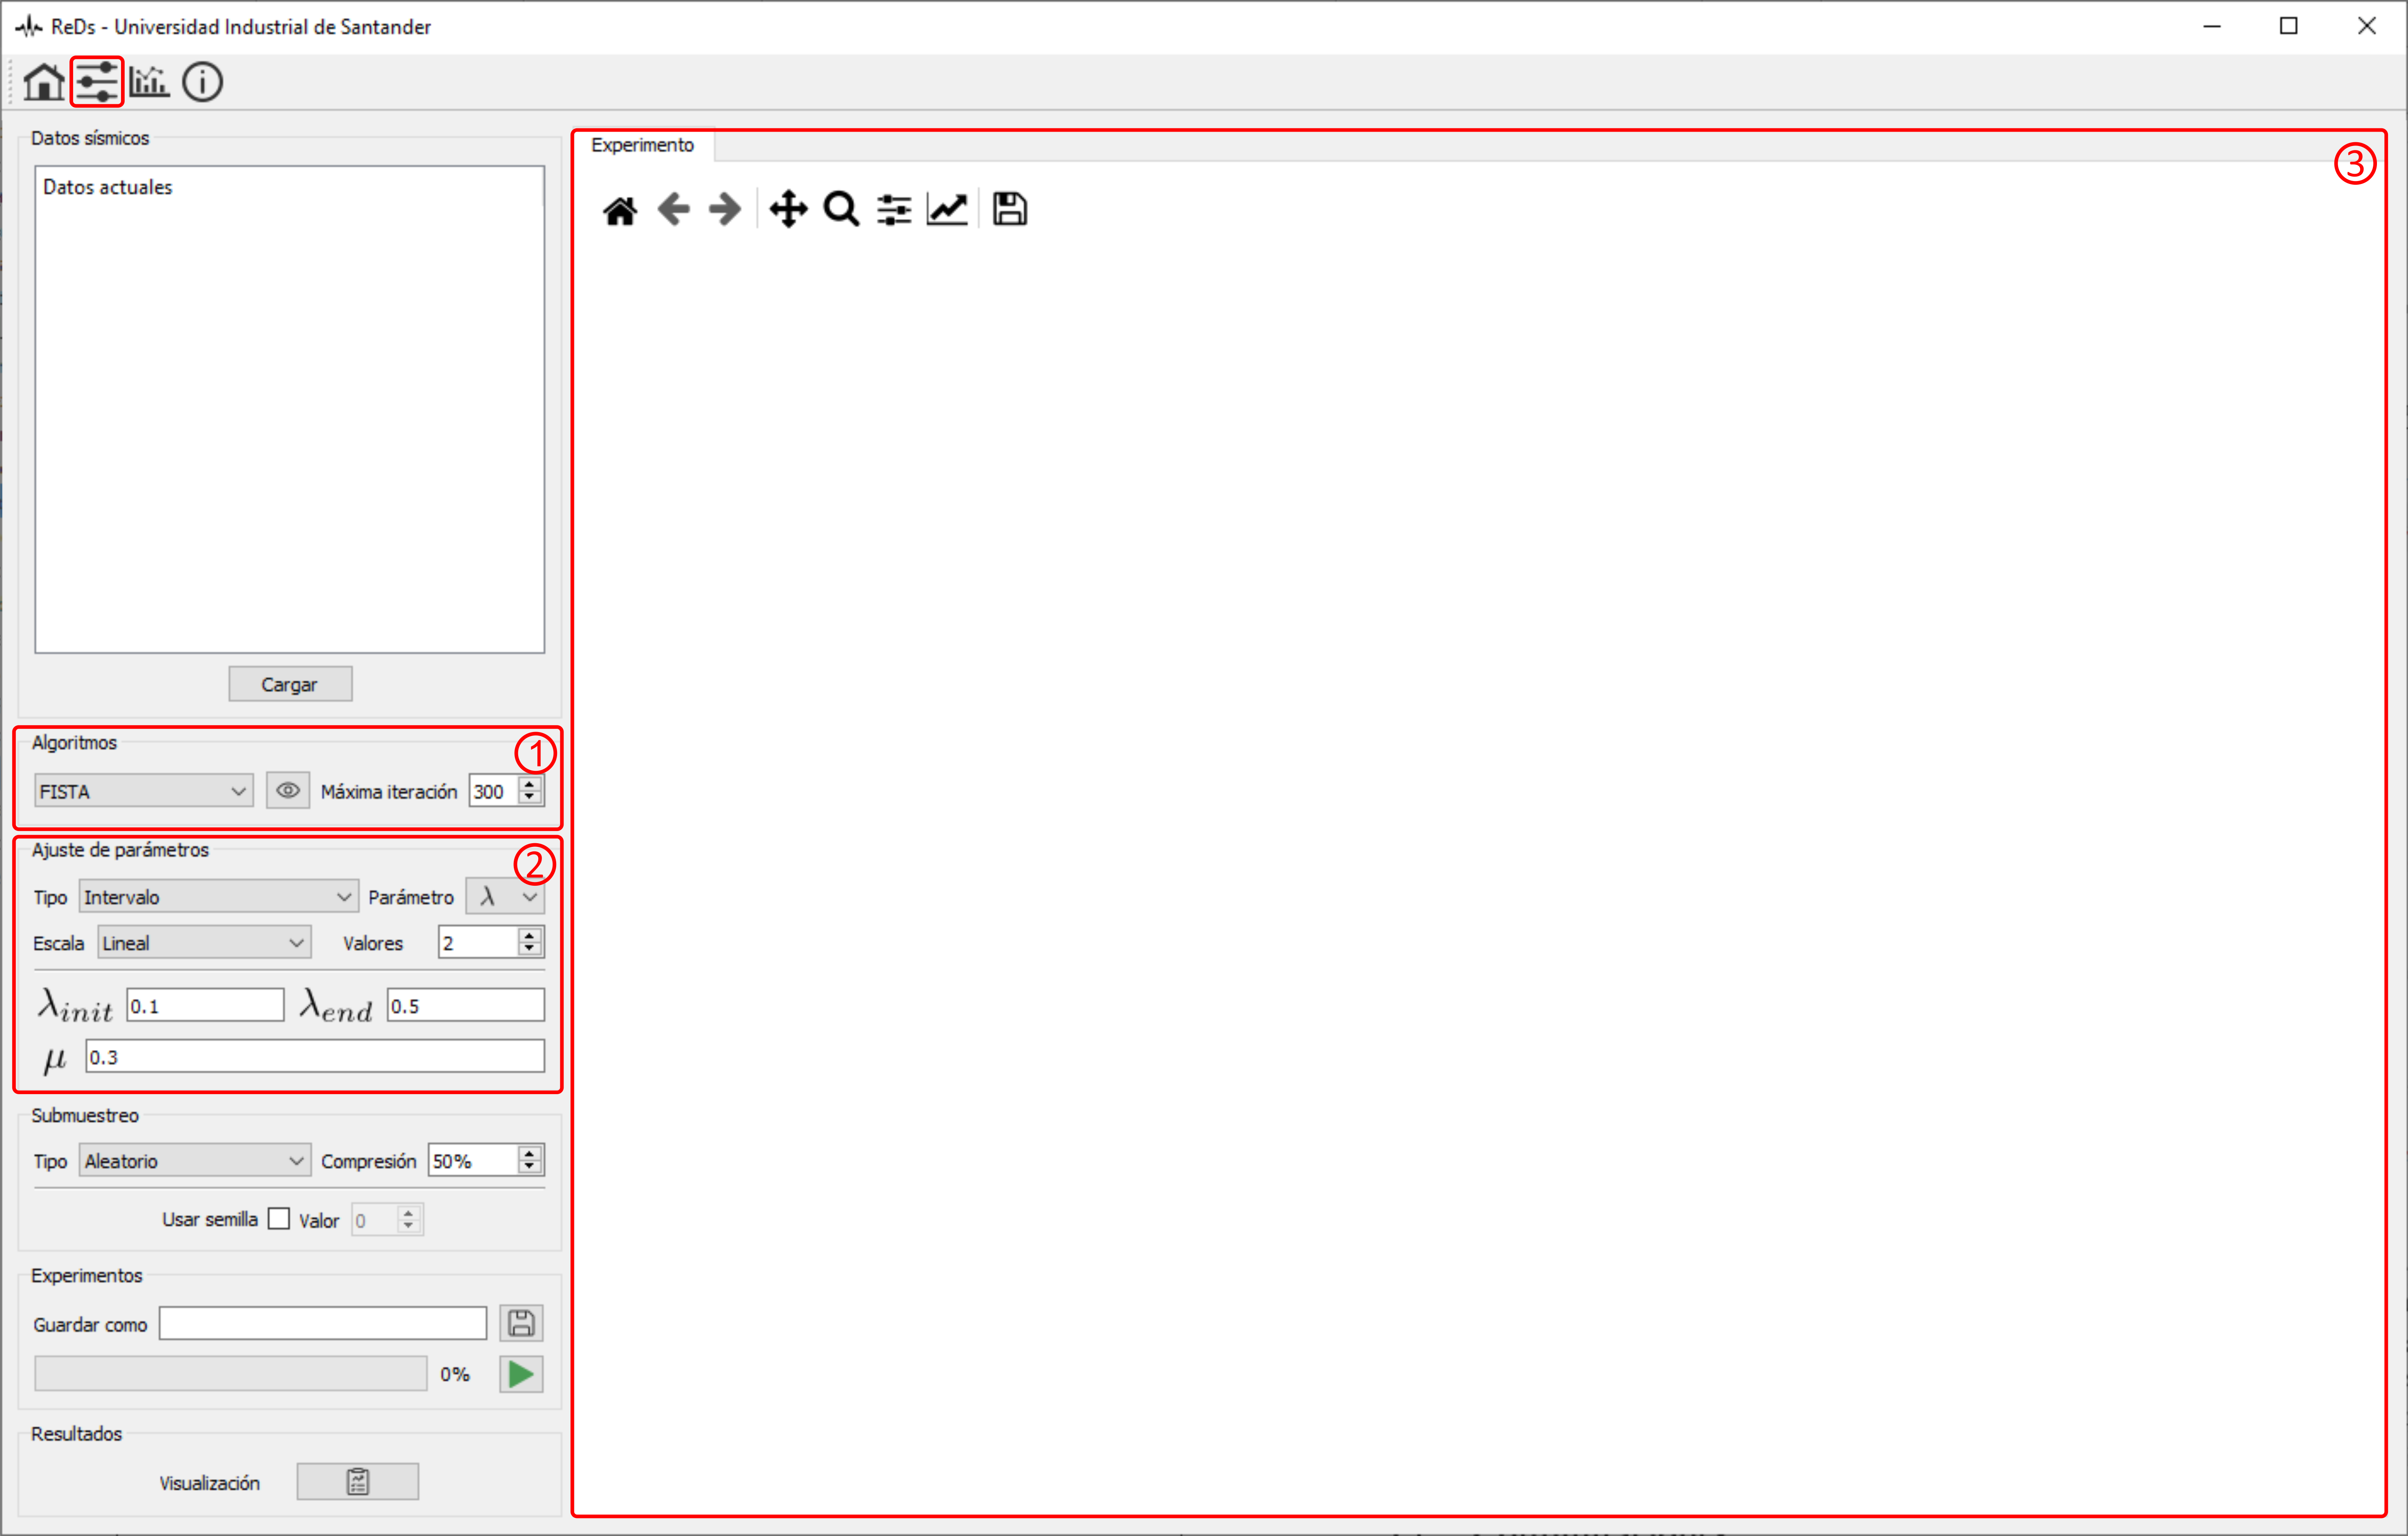
\includegraphics[width=1\linewidth]{tuning.png}
     \captionof{figure}{Partes del ajuste de parámetros en la aplicación.}
    \label{fig:tuning}
\end{Figure}

A continuación se listan los cambios que realiza la aplicación cuando se activa el modo de ajuste de parámetros:

\begin{dingautolist}{192}
	\setlength\itemsep{0em}
	\item Se deshabilita del panel de algoritmos los campos de asignación de parámetros para usar el nuevo de panel de ajuste de parámetros
	\item Se habilita el panel con los rangos y modos de ajuste de parámetros
	\item La visualización de resultados se simplifica a una sola gráfica
\end{dingautolist}

A continuación, se analiza el panel de ajuste de parámetros y la visualización de resultados.

\subsubsection{Configuraciones}

El panel de ajuste de parámetros, como se muestra en la figura \ref{fig:tuning_panel}, permite al usuario configurar el tipo de prueba que desea realizar. Se encuentra dividido en las siguientes secciones:

\begin{multicols}{2}
	
\begin{Figure}
	\centering
	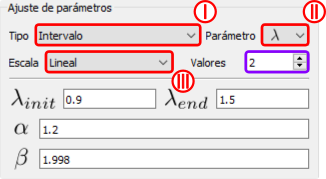
\includegraphics[width=0.9\linewidth]{tuning-panel.png}
	\captionof{figure}{Panel de ajuste de parámetros.}
	\label{fig:tuning_panel}
\end{Figure}	

\begin{itemize}
	
    \item[I.] \textbf{Tipo de ajuste:} Permite configurar la cantidad de valores de un mismo parámetro para algún algoritmo con los que se desean realizar pruebas. Este puede ser en intervalo, como se observa en la figura \ref{fig:tuning_panel}, donde el usuario debe ingresar la cantidad de \textcolor{ClearPurple}{\emph{valores}} que desea ingresar. El otro tipo de ajuste es de lista, donde el usuario debe ingresar cada uno de los valores con los que desea realizar pruebas.    
    
\end{itemize}

\end{multicols}

\begin{itemize}[leftmargin=0.5in]
	\setlength\itemsep{0em} 
	
	\item[II.] \textbf{Parámetro:} Este listado de parámetros se adaptará al algoritmo escogido. Su función es permitir al usuario seleccionar el parámetro que se quiere evaluar de acuerdo al tipo de ajuste.       
    
    \item[III.] \textbf{Escala:} Permite al usuario modificar el comportamiento de los valores de los parámetros. Esta escala puede ser lineal, cuyo comportamiento no afectará a los valores de los parámetros, de tal manera que $y = x$, donde $x$ es cualquier valor de los parámetros. El otro tipo de escala es la escala logarítmica, la cual tomará cada uno de los valores establecidos por el usuario, de tal manera que $y = 10^x$.
    
\end{itemize}

\subsubsection*{Realizando un ajuste de parámetros óptimo}

Para realizar un ajuste de parámetros óptimo, primero se deberá cargar el dato sísmico, tal como se indica en la sección \ref{sec:data_lecture}.

\begin{multicols}{2}

Ahora, se debe seleccionar el algoritmo al cual se le desea hallar los parámetros óptimos dado el dato sísmico cargado. Para este ejemplo se selecciona el algoritmo FISTA, y se establece la configuración de parámetros que se observa en la figura \ref{fig:tuning_params}. A continuación se explica la selección de parámetros:

\begin{itemize}
    \item Para el ajuste de parámetros se seleccionó de tipo intervalo con escala logarítmica ya que facilita al usuario la selección de parámetros y visualización de resultados obtenidos.
    \item Para el submuestreo se fijó una semilla con el propósito de que la muestra sísmica siempre tenga el mismo tipo de submuestreo y poder hacer una óptima selección de los parámetros.
\end{itemize}

\begin{Figure}
    \centering
    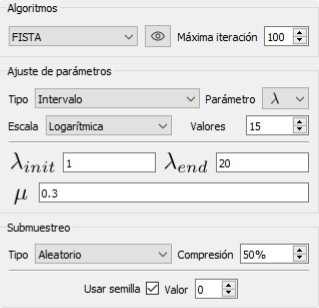
\includegraphics[width=1\linewidth]{tuning-params.png}
     \captionof{figure}{Ajuste de parámetros para el algoritmo FISTA.}
    \label{fig:tuning_params}
\end{Figure}

\end{multicols}

Una vez completada la configuración se procede a ajustar el parámetro $\lambda$. Los resultados se observan en la figura \ref{fig:tuning_1}. En esta figura se pueden observar los resultados obtenidos para la configuración de parámetros establecida en la figura \ref{fig:tuning_params}. Por inspección, el valor óptimo para $\lambda$ es $\lambda^* \approx 2.91$.

\begin{Figure}
    \centering
    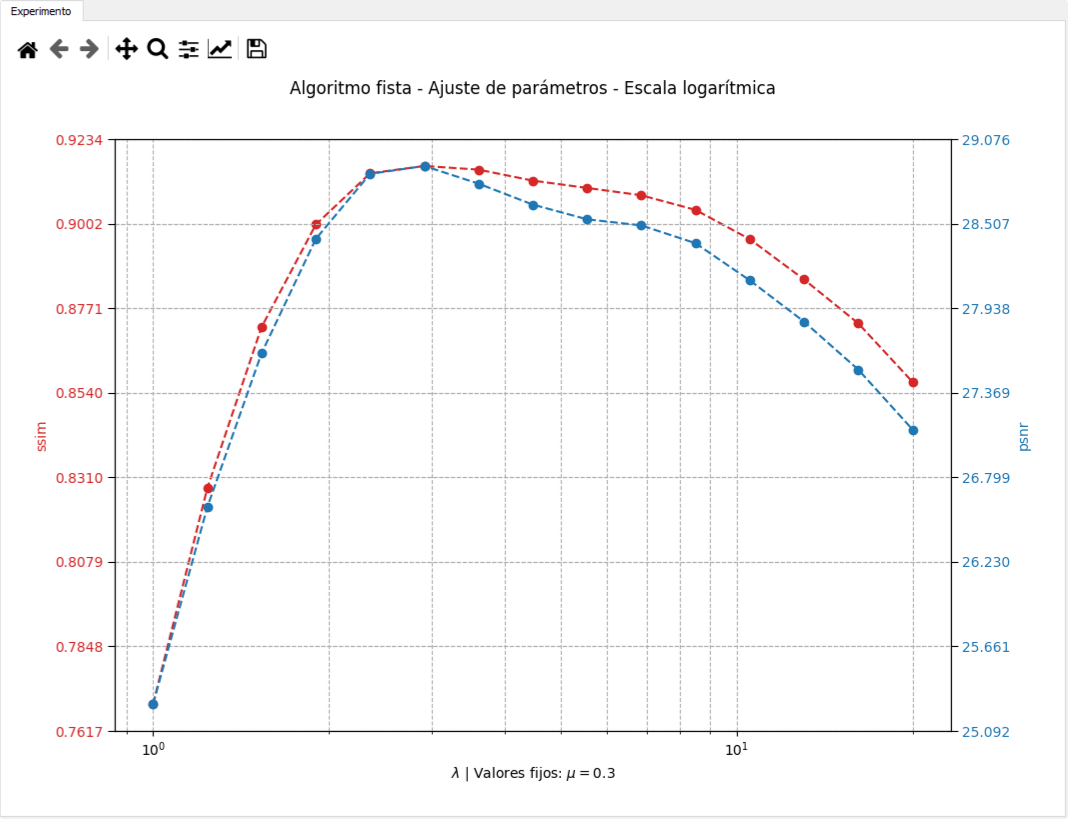
\includegraphics[width=1\linewidth]{tuning-1.png}
     \captionof{figure}{Ajuste del parámetro $\lambda$ para el algoritmo FISTA.}
    \label{fig:tuning_1}
\end{Figure}

\begin{multicols}{2}
	
\begin{Figure}
	\centering
	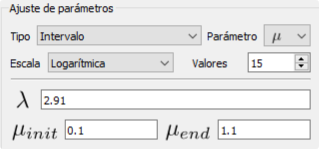
\includegraphics[width=0.8\linewidth]{tuning-params-2.png}
	\captionof{figure}{Ajuste del parámetro $\mu$ para el algoritmo FISTA.}
	\label{fig:tuning_params_2}
\end{Figure}

Ahora, para encontrar el valor óptimo $\mu^*$, se toma el valor de $\lambda^*$ y se evalua para un intervalo de $\mu$, como el que se observa en la figura \ref{fig:tuning_params_2}. Los resultados obtenidos para este ajuste de parámetros se observan en la figura \ref{fig:tuning_2}. Por inspección, se observa que el valor óptimo $\mu^* \approx 0.39$.

\end{multicols}

\begin{Figure}
    \centering
    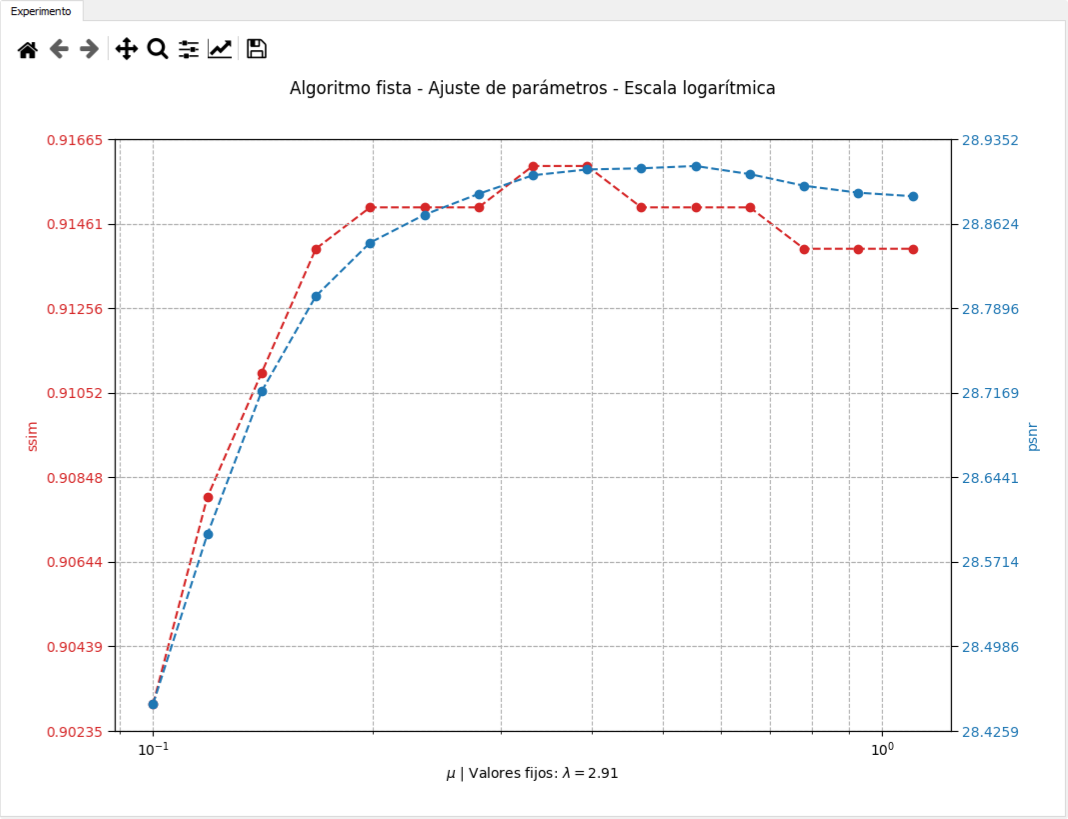
\includegraphics[width=1\linewidth]{tuning-2.png}
     \captionof{figure}{Ajuste del parámetro $\mu$ para el algoritmo FISTA.}
    \label{fig:tuning_2}
\end{Figure}

\subsection{Modo Comparación de Algoritmos}

\begin{multicols}{2}

El tercer modo de ejecución de ReDs permite correr los cuatro algoritmos de reconstrucción al mismo tiempo. Este modo se activa con el tercer botón del menú principal, tal como se muestra en la figura \ref{fig:comp}. El objetivo es realizar comparaciones entre los algoritmos de reconstrucción.
\vfill\null
\columnbreak
\begin{Figure}
	\centering
	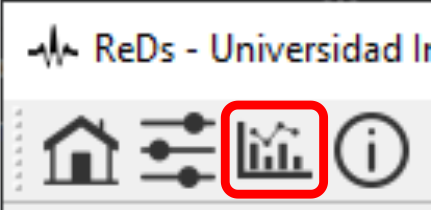
\includegraphics[width=0.4\linewidth]{comp-tab.png}
	\captionof{figure}{Modo de comparación de algoritmos.}
	\label{fig:comp}
\end{Figure}
\end{multicols}
Al igual que con el modo de ajuste de parámetros, el modo de comparación modifica la interfaz gráfica, tal y como se muestra en la figura \ref{fig:main-comp}. A continuación se listan los cambios que realiza la aplicación cuando se activa el modo de comparación de algoritmos:

\begin{dingautolist}{192}
	\setlength\itemsep{0em}
	\item Se presentan los cuatro algoritmos de reconstrucción, con sus parámetros
	\item La visualización de resultados se simplifica a una sola gráfica
\end{dingautolist}

\begin{Figure}
	\centering
	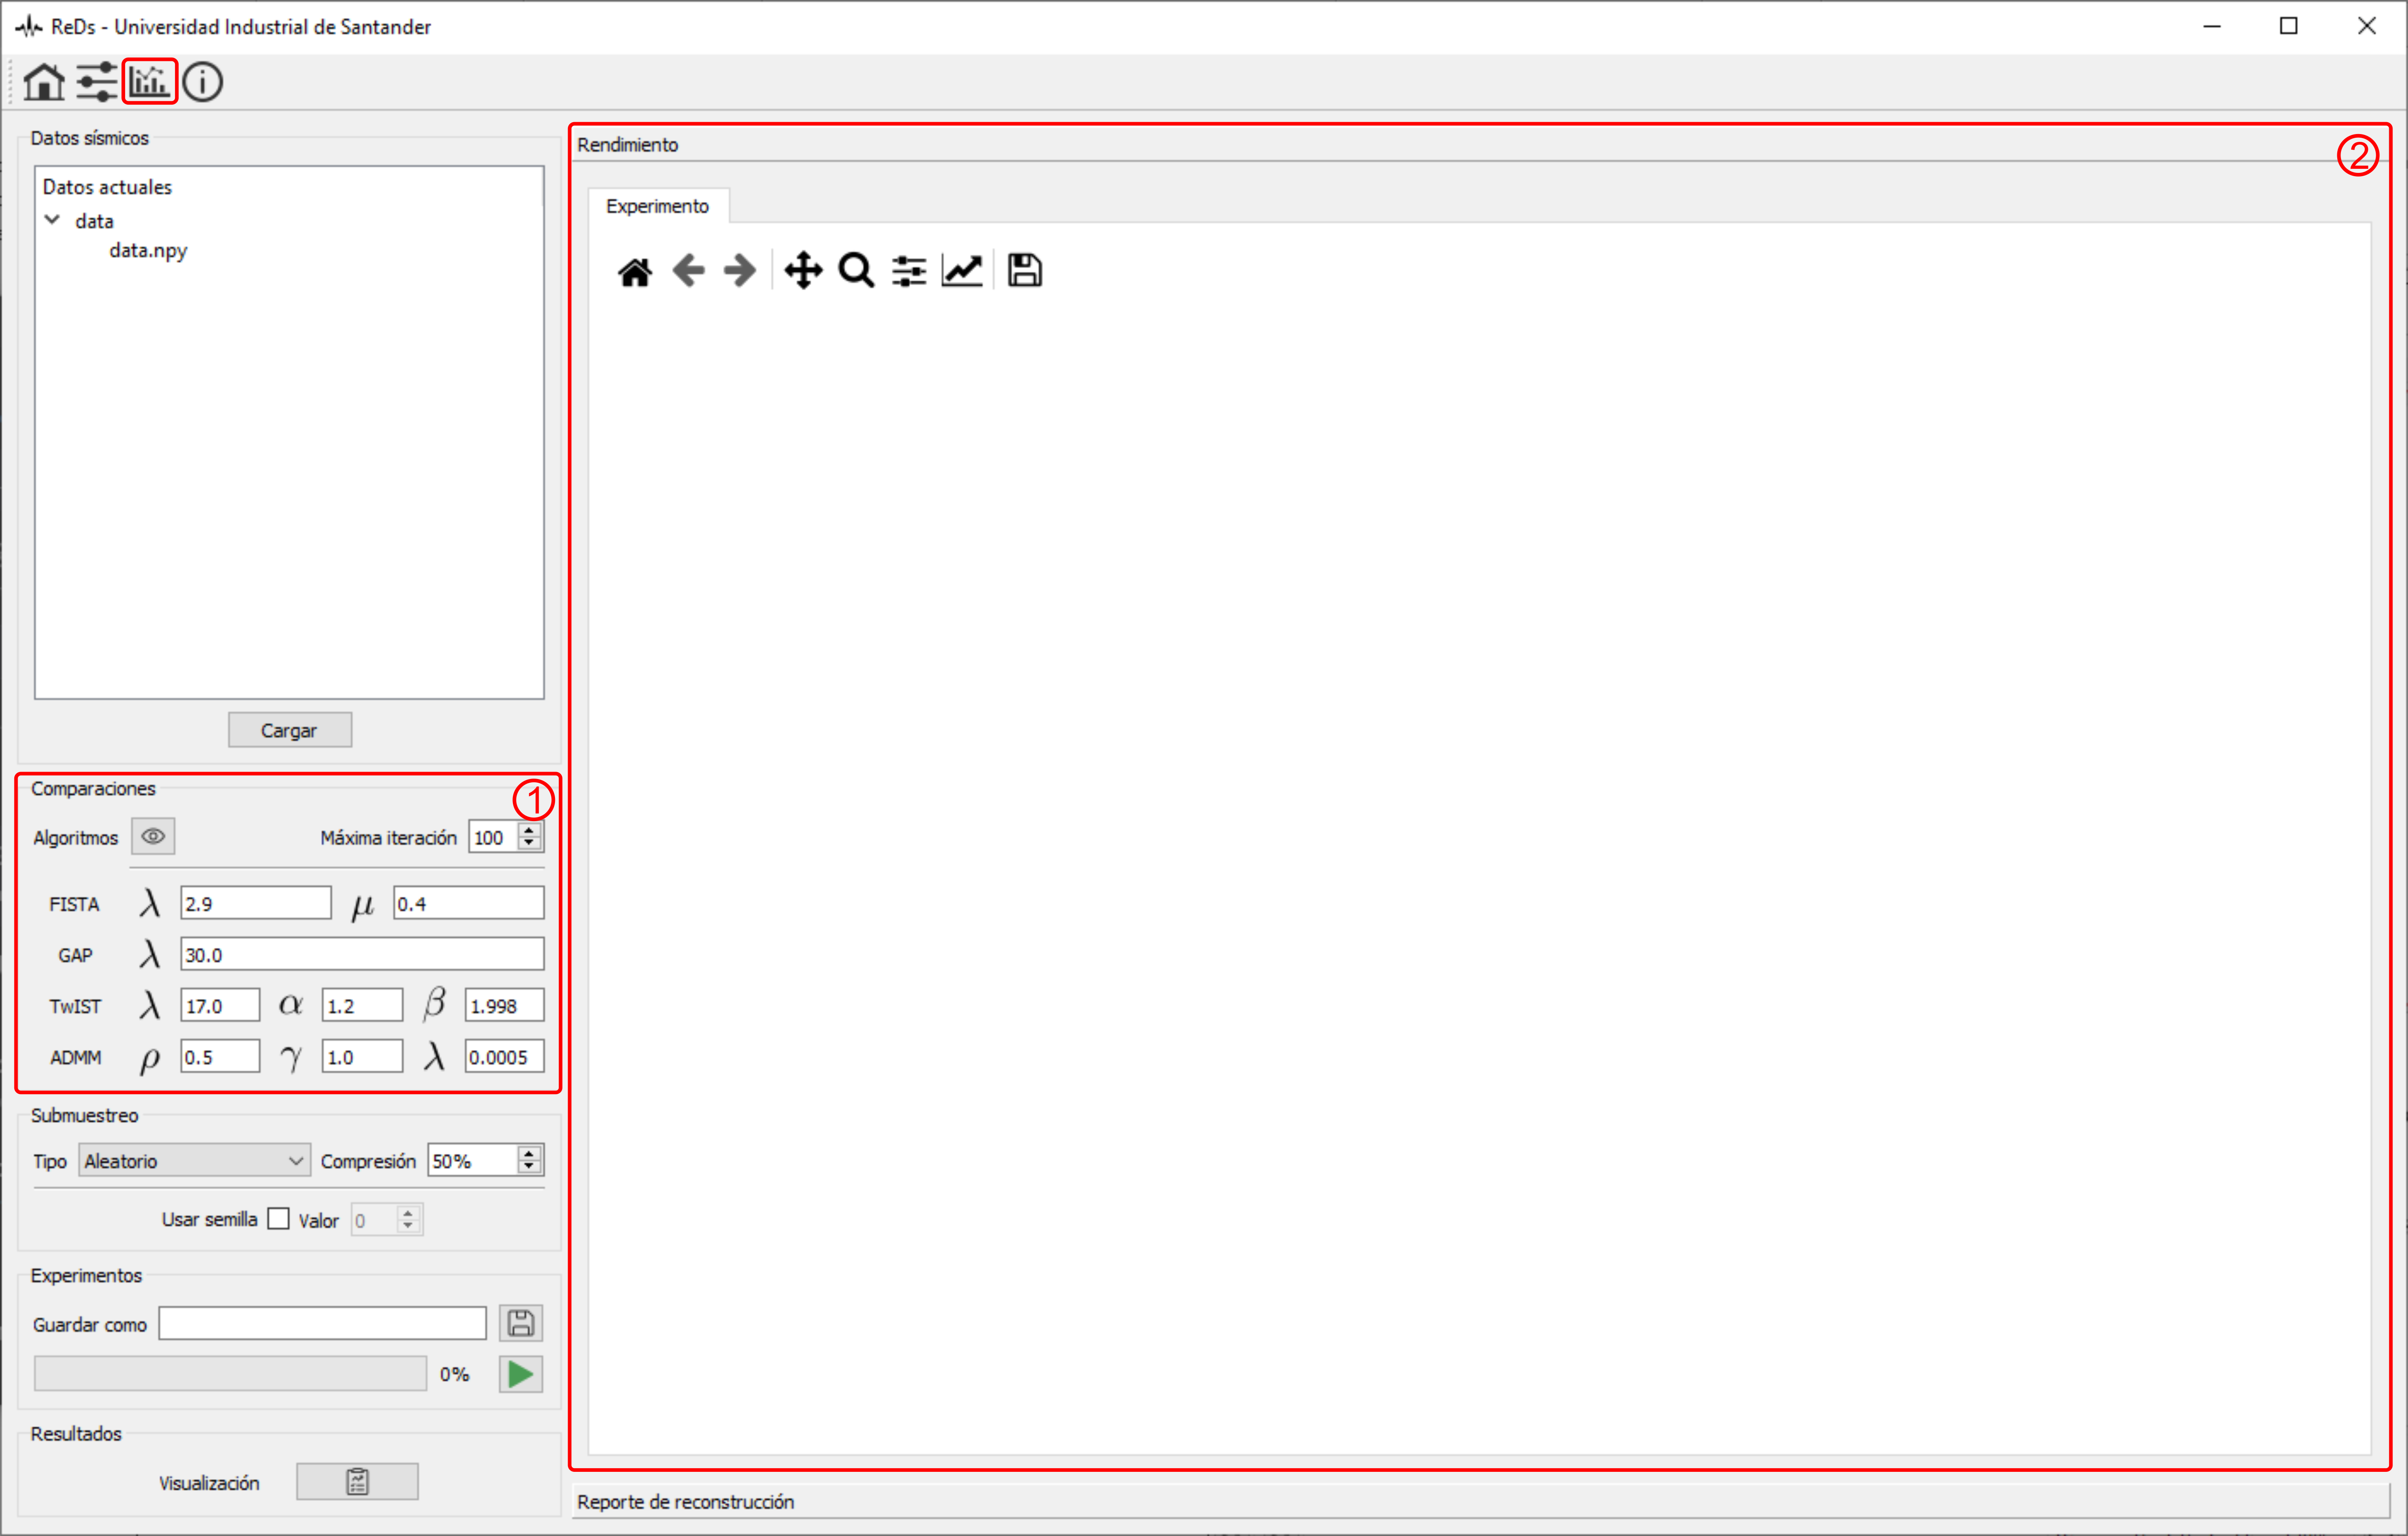
\includegraphics[width=0.85\linewidth]{main-comp.png}
	\captionof{figure}{Interfaz modo de comparación de algoritmos.}
	\label{fig:main-comp}
\end{Figure}

A continuación, se analiza el panel de comparación de algoritmos y la visualización de resultados para este modo.

\subsubsection{Configuraciones}

El panel comparación de algoritmos, como se muestra en la figura \ref{fig:comp_panel}, permite al usuario configurar el tipo de prueba que desea realizar. Se encuentra dividido en las siguientes secciones:

\begin{multicols}{2}
	
	\begin{Figure}
		\centering
		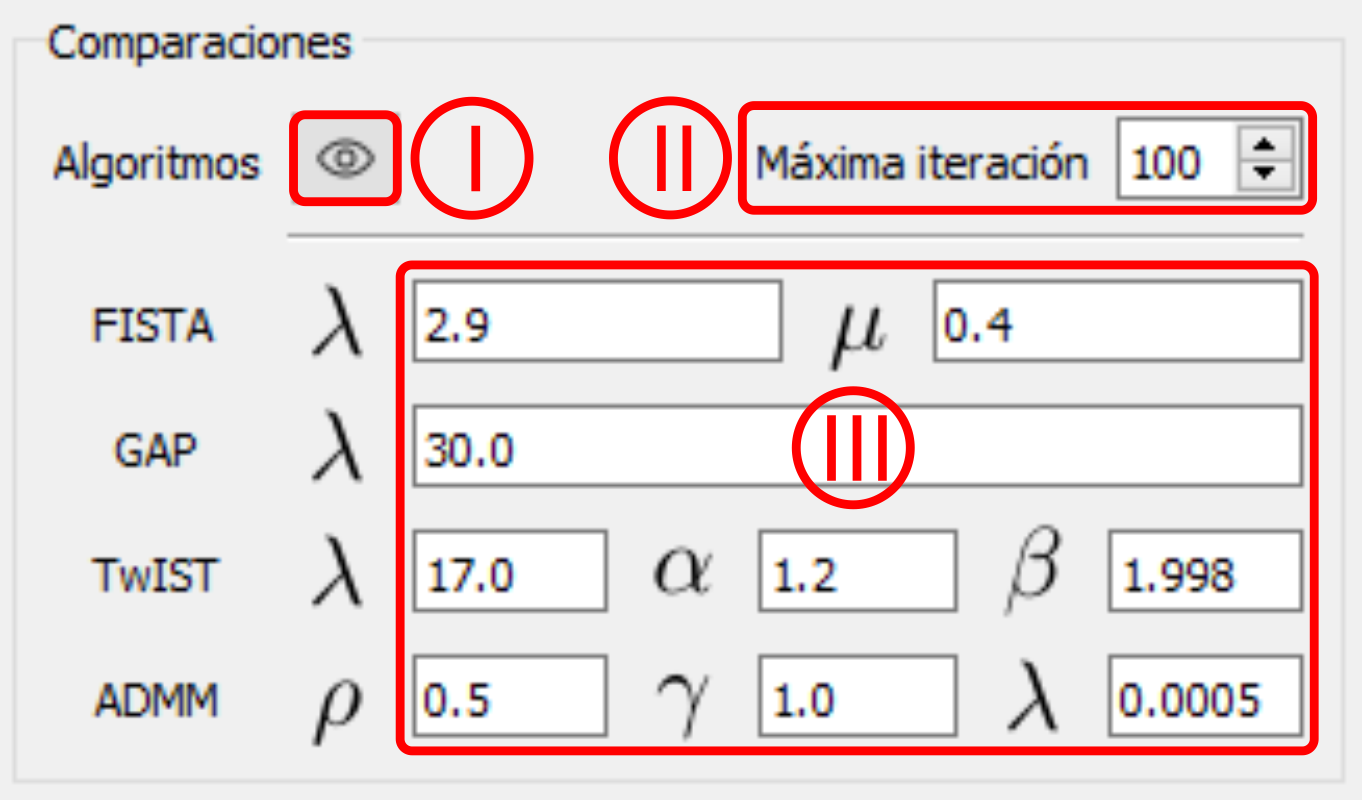
\includegraphics[width=0.9\linewidth]{comp-panel.png}
		\captionof{figure}{Panel de ajuste de parámetros.}
		\label{fig:comp_panel}
	\end{Figure}	
	
	\begin{itemize}
		
		\item[I.] \textbf{Ver Ecuaciones:} Muestra las ecuaciones de los cuatro algoritmos de ajuste, con sus parámetros.
		\item[II.] \textbf{Maximo de Iteraciones:} Define el número máximo de iteraciones para todos los cuatro algoritmos, por igual.
		\item[III.] \textbf{Parámetros:} Se definen los parámetros para todos y cada uno de los algoritmos de reconstrucción, al igual que en el numeral 2.2.
		
	\end{itemize}
	
\end{multicols}

\subsubsection*{Realizando una comparación de algoritmos}

Para realizar una comparación de algoritmos primero se deberá cargar el dato sísmico, tal como se indica en la sección \ref{sec:data_lecture}.

Ahora, se deben ingresar los valores para cada uno de los parámetros de los cuatro algoritmos de reconstrucción. En total son 9 parámetros a establecer: 2 para FISTA, 1 para GAP, 3 para TwIST y 3 para ADMM.

Por último definimos el número de iteraciones, en 300, el tipo de submuestreo, aleatorio con 50\% de compresión, y el archivo de salida de resultados, tal como se muestra en la sección 2.4.1. Para correr el experimento se debe pulsar en el botón \hspace{0.5mm} \faPlay \hspace{0.5mm}.

Una vez termina la ejecución de los cuatro algoritmos, se presentan los resultados de las cuatro reconstrucciones en las pestañas Rendimiento y Reporte de reconstrucción, tal como se muestra en las figuras \ref{fig:result-comp1} y \ref{fig:result-comp2} respectivamente.

\begin{Figure}
	\centering
	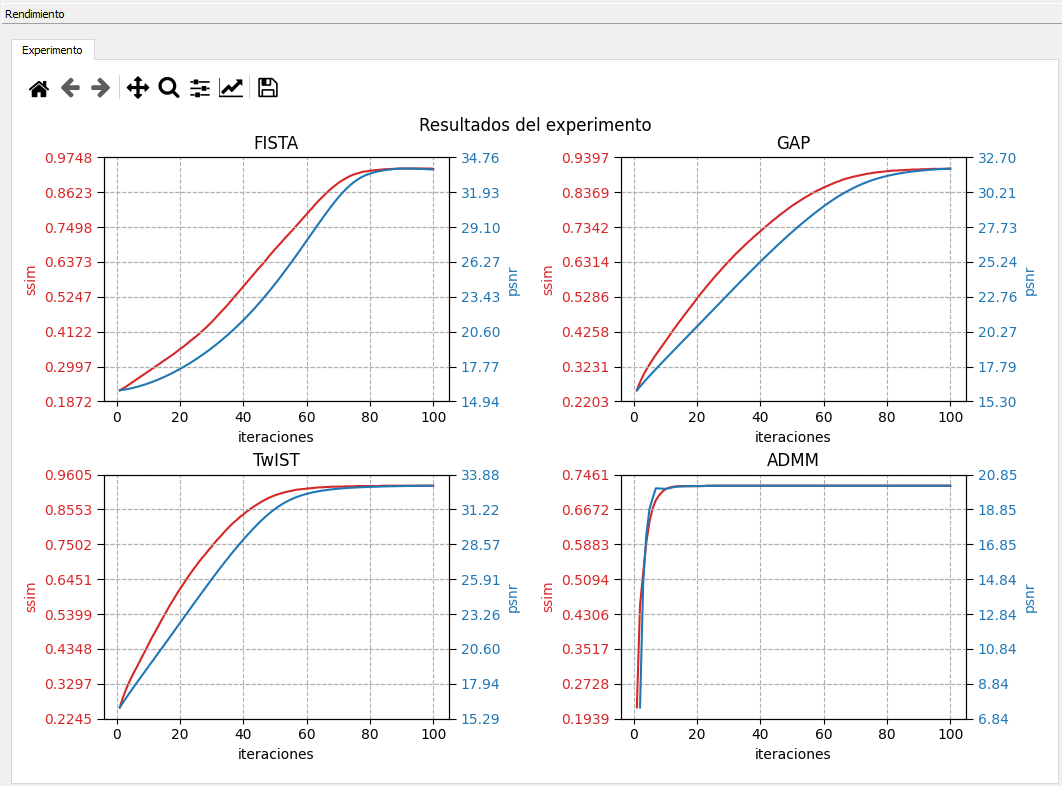
\includegraphics[width=0.8\linewidth]{result-comp1.png}
	\captionof{figure}{Rendimiento de la comparación de algoritmos}
	\label{fig:result-comp1}
\end{Figure}

\begin{Figure}
	\centering
	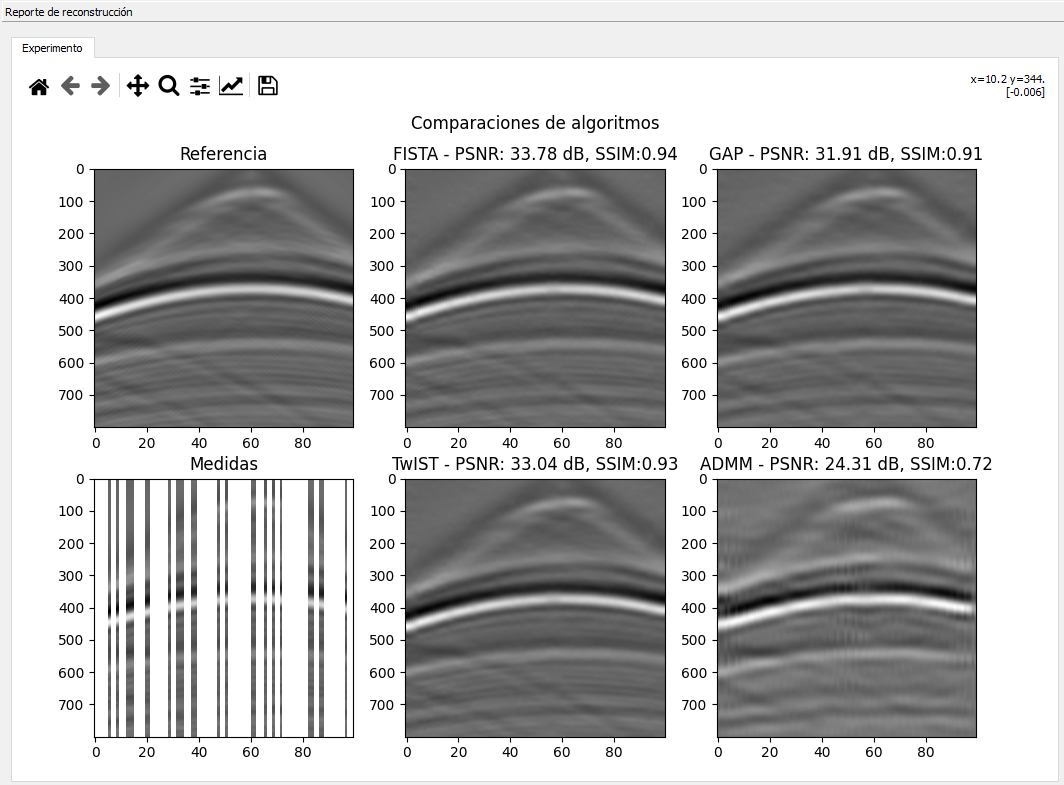
\includegraphics[width=0.8\linewidth]{result-comp2.png}
	\captionof{figure}{Reporte de reconstrucción de la comparación de algoritmos}
	\label{fig:result-comp2}
\end{Figure}

\subsection{Visualización general de Resultados}

Los experimentos realizados quedan almacenados en el directorio escogidos por el usuario de forma local en su computadora. Esos resultados pueden ser visualizados a través del panel de visualización \circled{6} en el extremo inferior izquierdo de la figura \ref{fig:vision}.

\subsubsection{Menú principal}

\begin{multicols}{2}

Esta herramienta funciona de la misma manera para los dos tipos de experimentos actuales (general y ajuste de parámetros), cargando los respectivos datos como se visualizaron en secciones anteriores. Para usar este panel debemos pulsar el botón en \circled{1}, como se observa en la figura \ref{fig:report_1}. Al pulsar este botón el comportamiento de la interfaz cambiará a lectura de resultados de experimentos ya realizados. Por lo que ahora se usará el botón \emph{Cargar} \circled{2} para cargar dichos datos.

\begin{Figure}
    \centering
    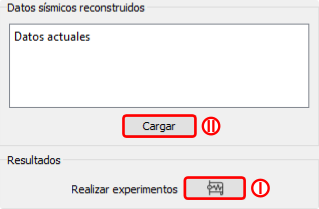
\includegraphics[width=0.8\linewidth]{report-1.png}
     \captionof{figure}{Lectura de resultados.}
    \label{fig:report_1}
\end{Figure}

\end{multicols}

\textbf{Leyendo resultados de experimentos realizados}

\begin{multicols}{2}

\begin{Figure}
	\centering
	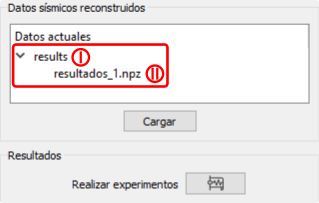
\includegraphics[width=0.8\linewidth]{report-3.png}
	\captionof{figure}{Panel con resultados cargados de un experimento previo.}
	\label{fig:report_3}
\end{Figure}

Como se observa en la figura \ref{fig:report_2}, el usuario podrá seleccionar el archivo que desee visualizar (en este caso \emph{resultados\_1.npz}) con los resultados de un experimento previamente realizado. Una vez seleccionado, se debe pulsar la opción \emph{Abrir} y los resultados serán cargados tanto en el panel de resultados de la figura \ref{fig:report_3}, donde \circled{I} ese el directorio padre del los resultados cargados \circled{II}.

\end{multicols}

\begin{Figure}
    \centering
    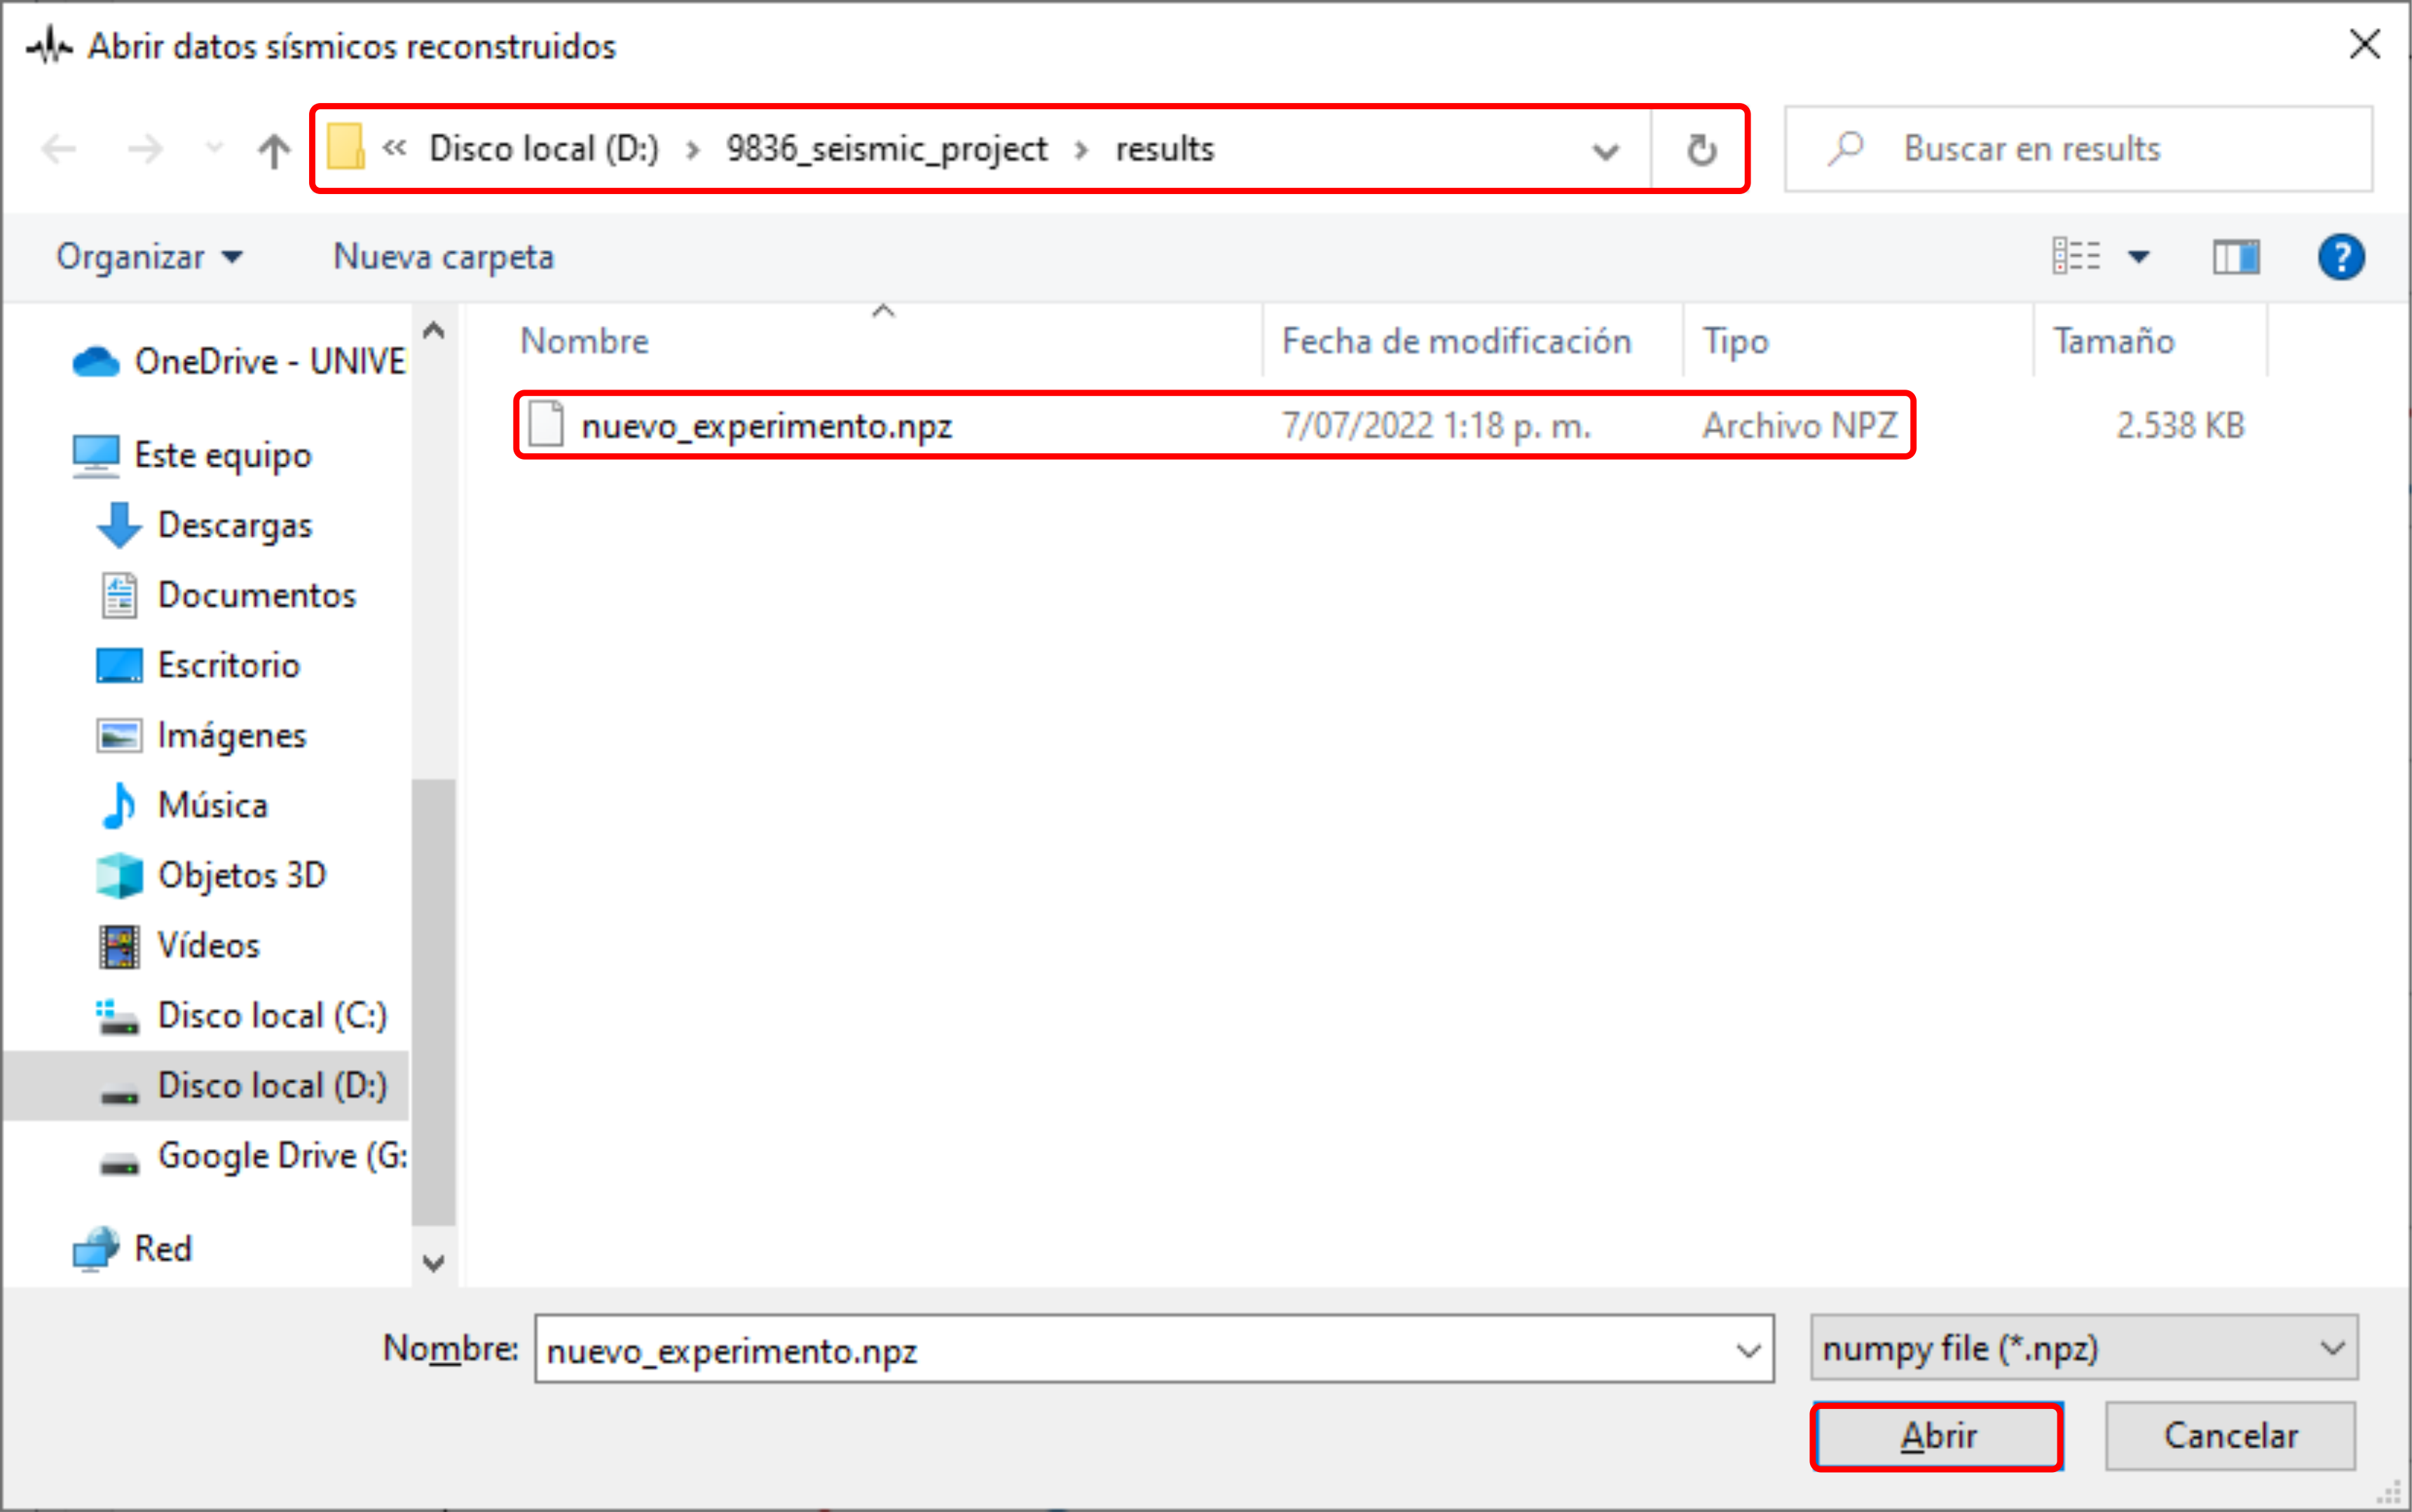
\includegraphics[width=0.9\linewidth]{report-2.png}
     \captionof{figure}{Ventana de selección de resultados.}
    \label{fig:report_2}
\end{Figure}

Finalmente, los datos cargados se pueden visualizar en el panel de gráficas a la derecha de la aplicación, como se observa en la figura \ref{fig:report_4}.

\subsubsection{Menú de ajuste de parámetros}

Similar al proceso de lectura de datos para experimentos realizados en el menú principal, para esta ocasión se debe estar en el menú de ajuste de parámetros, como se muestra en la figura \ref{fig:tuning}, y repetir el proceso explicado previamente pero cargando los resultados de algún experimento de ajuste de parámetros. A modo de ejemplo, se cargó el archivo de resultados \emph{resultados\_2.npz}, tal como se visualiza en la figura \ref{fig:report_5}. Este modo es exclusivamente de visualización y no permite modificar el rango de valores evaluados.

\begin{Figure}
    \centering
    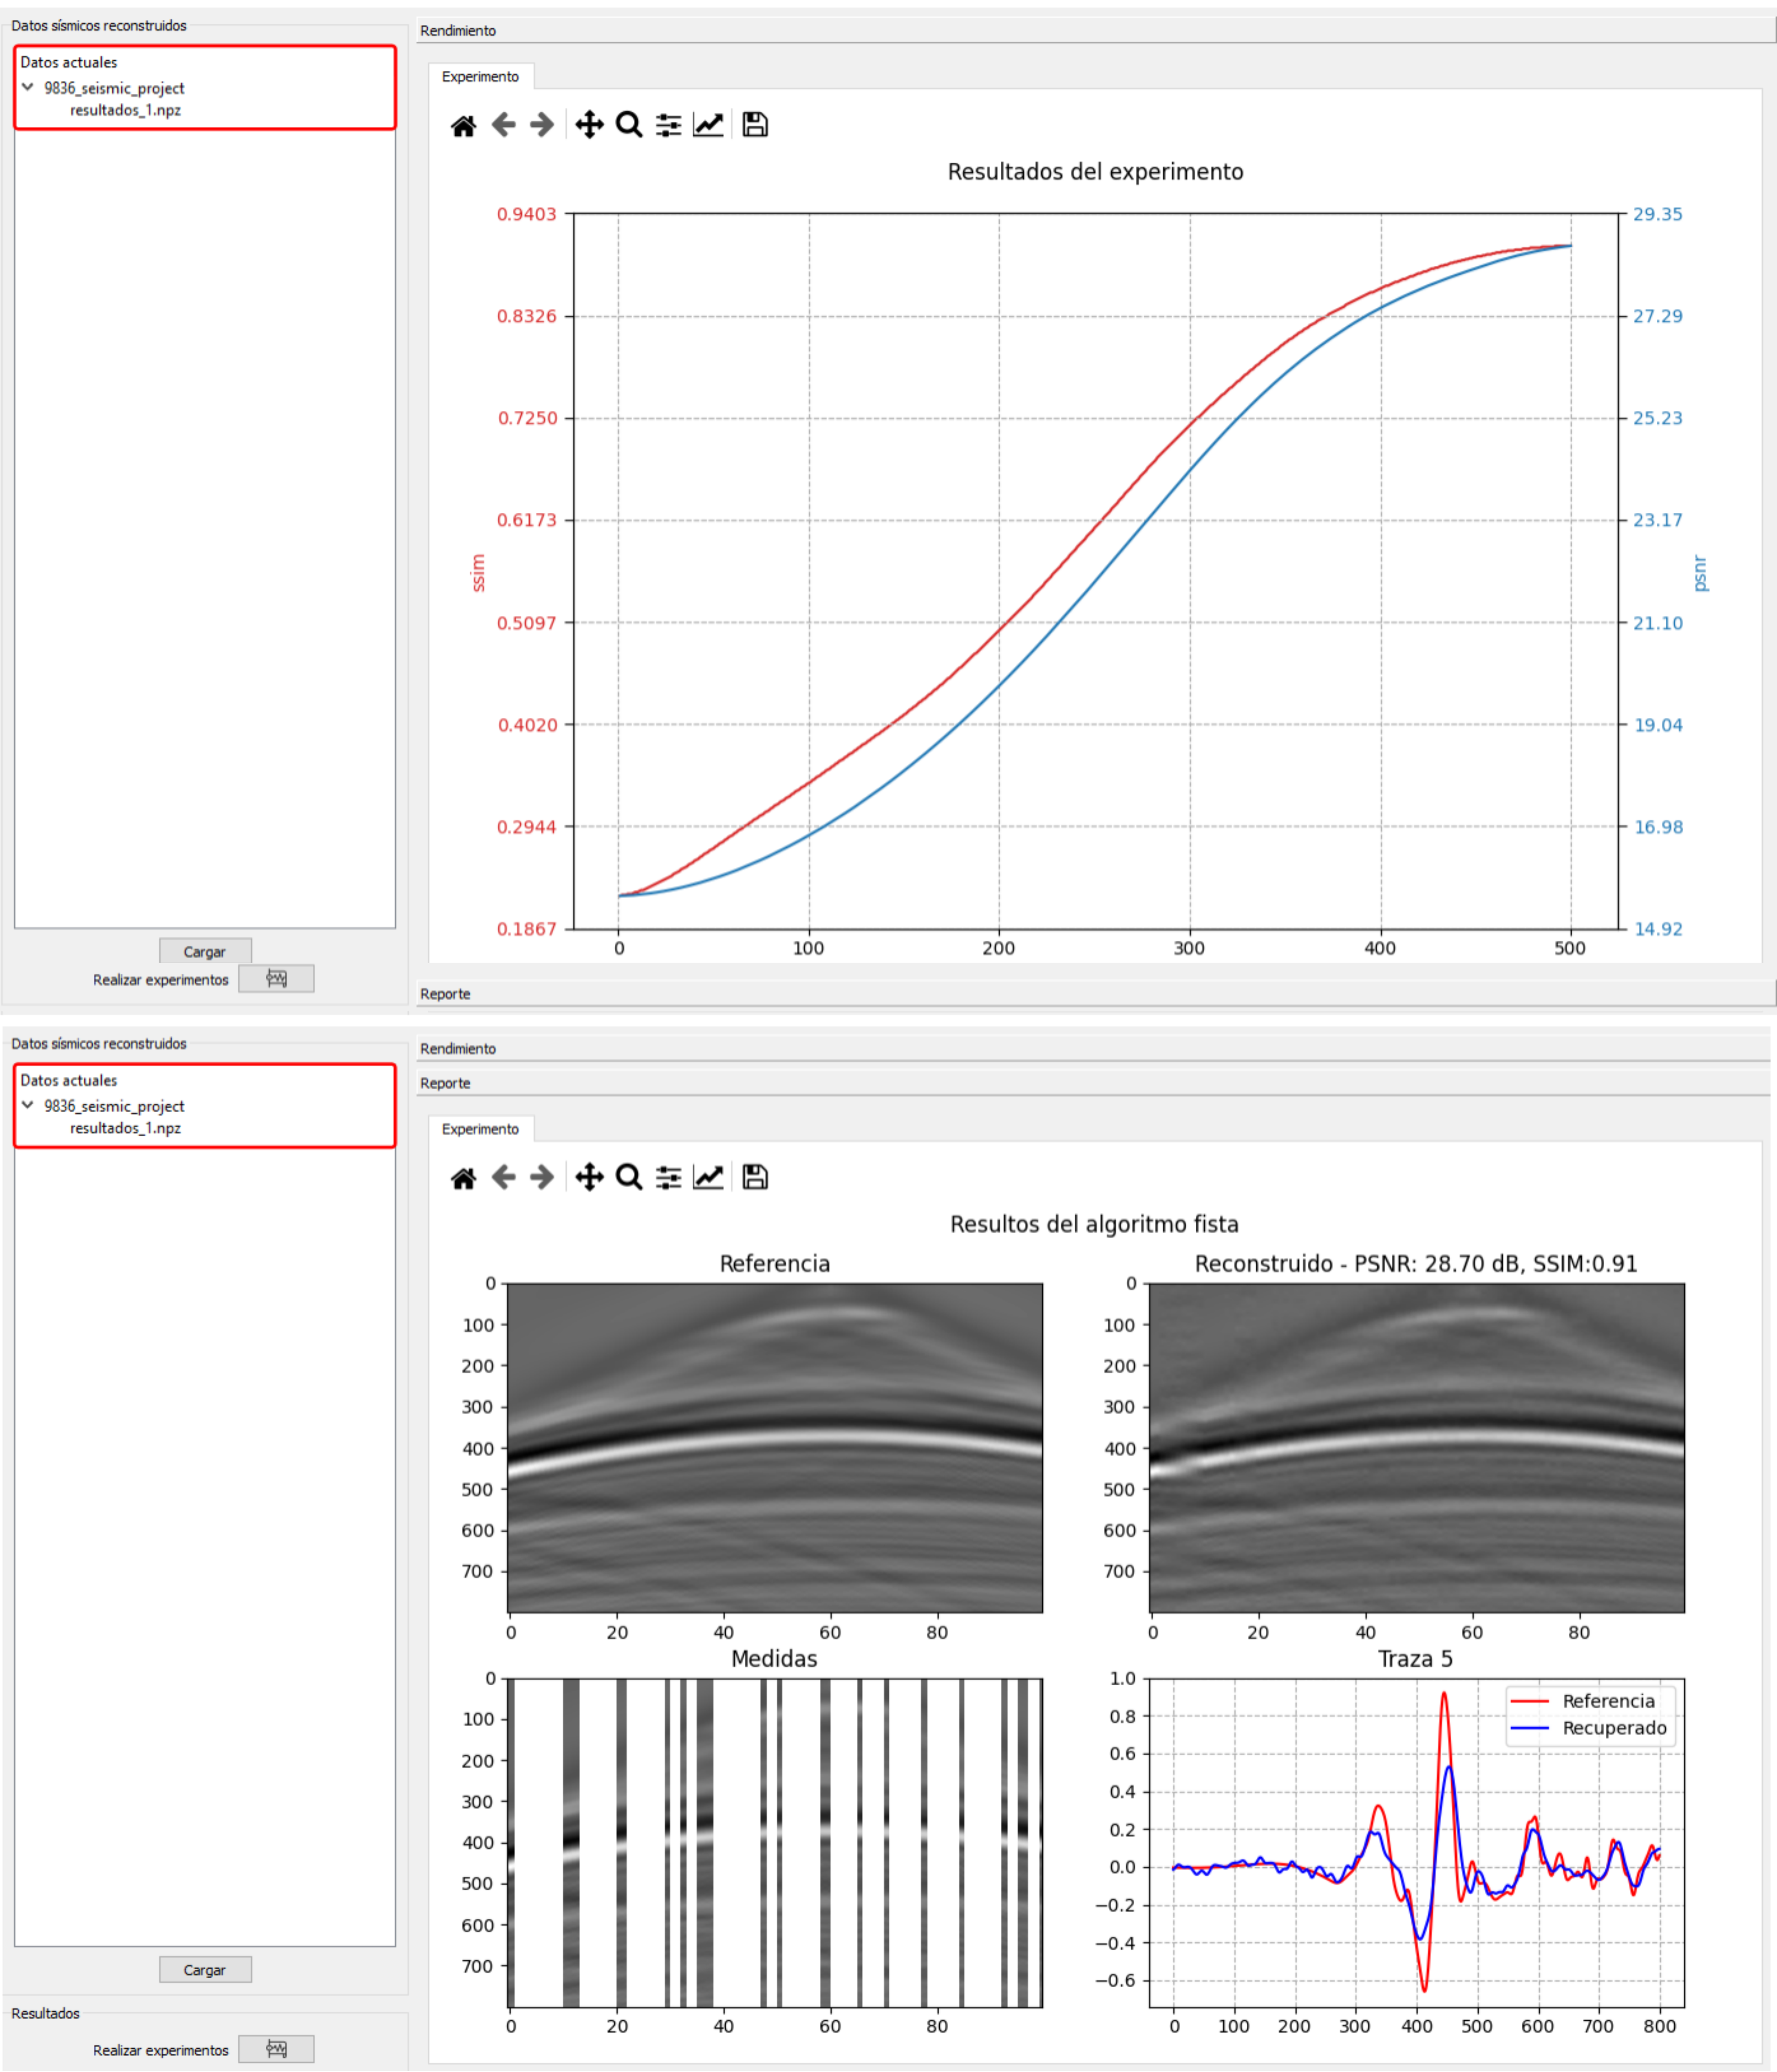
\includegraphics[width=1\linewidth]{report-4.png}
     \captionof{figure}{Visualización de los resultados cargados.}
    \label{fig:report_4}
\end{Figure}

\begin{Figure}
    \centering
    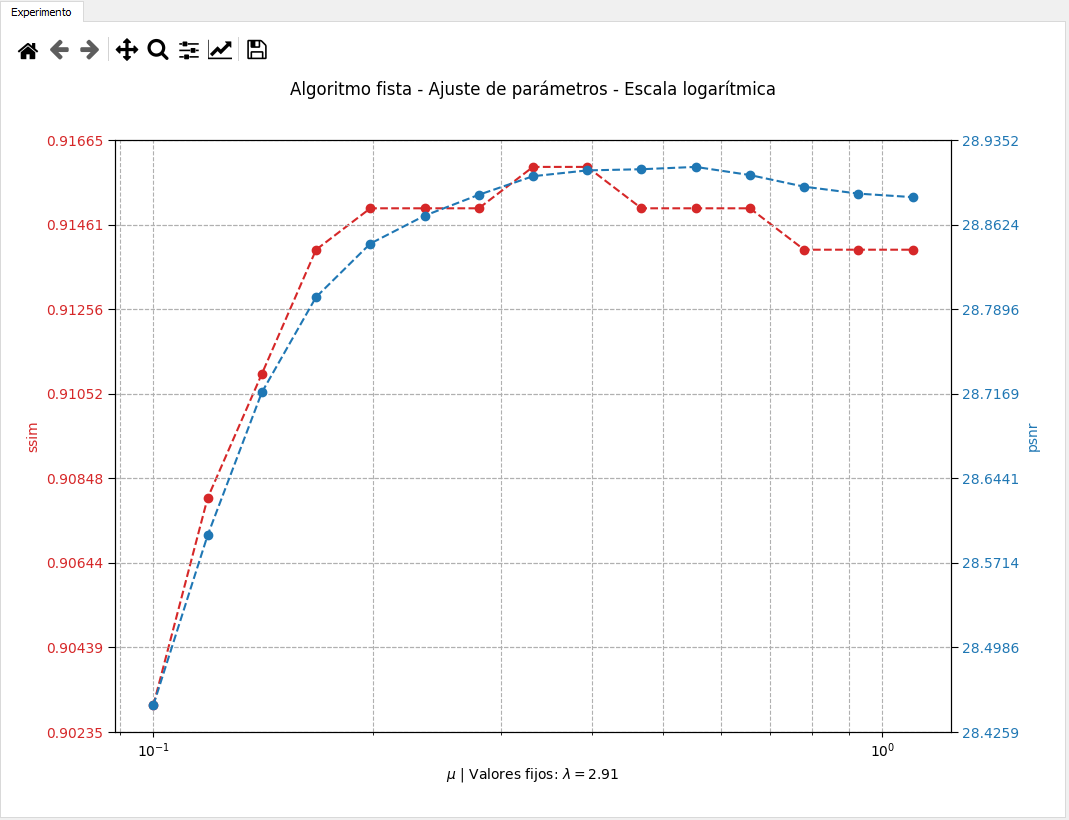
\includegraphics[width=1\linewidth]{report-5.png}
     \captionof{figure}{Visualización de los resultados de ajuste de parámetros cargados.}
    \label{fig:report_5}
\end{Figure}

\subsubsection{Menú de comparación de algoritmos}

Por último, es posible cargar resultados de comparaciones de algoritmos. Para esto habilitamos el modo \textit{Comparación de Algoritmos} (ver figura \ref{fig:comp}), y presionamos el botón \textit{Ver Resultados} en la parte inferior izquierda. A modo de ejemplo, se cargó el archivo de resultados \emph{results\_comp.npz}, tal como se visualiza en la figura \ref{fig:report_6}. Este modo es exclusivamente de visualización y no permite modificar el rango de valores evaluados.

\begin{Figure}
	\centering
	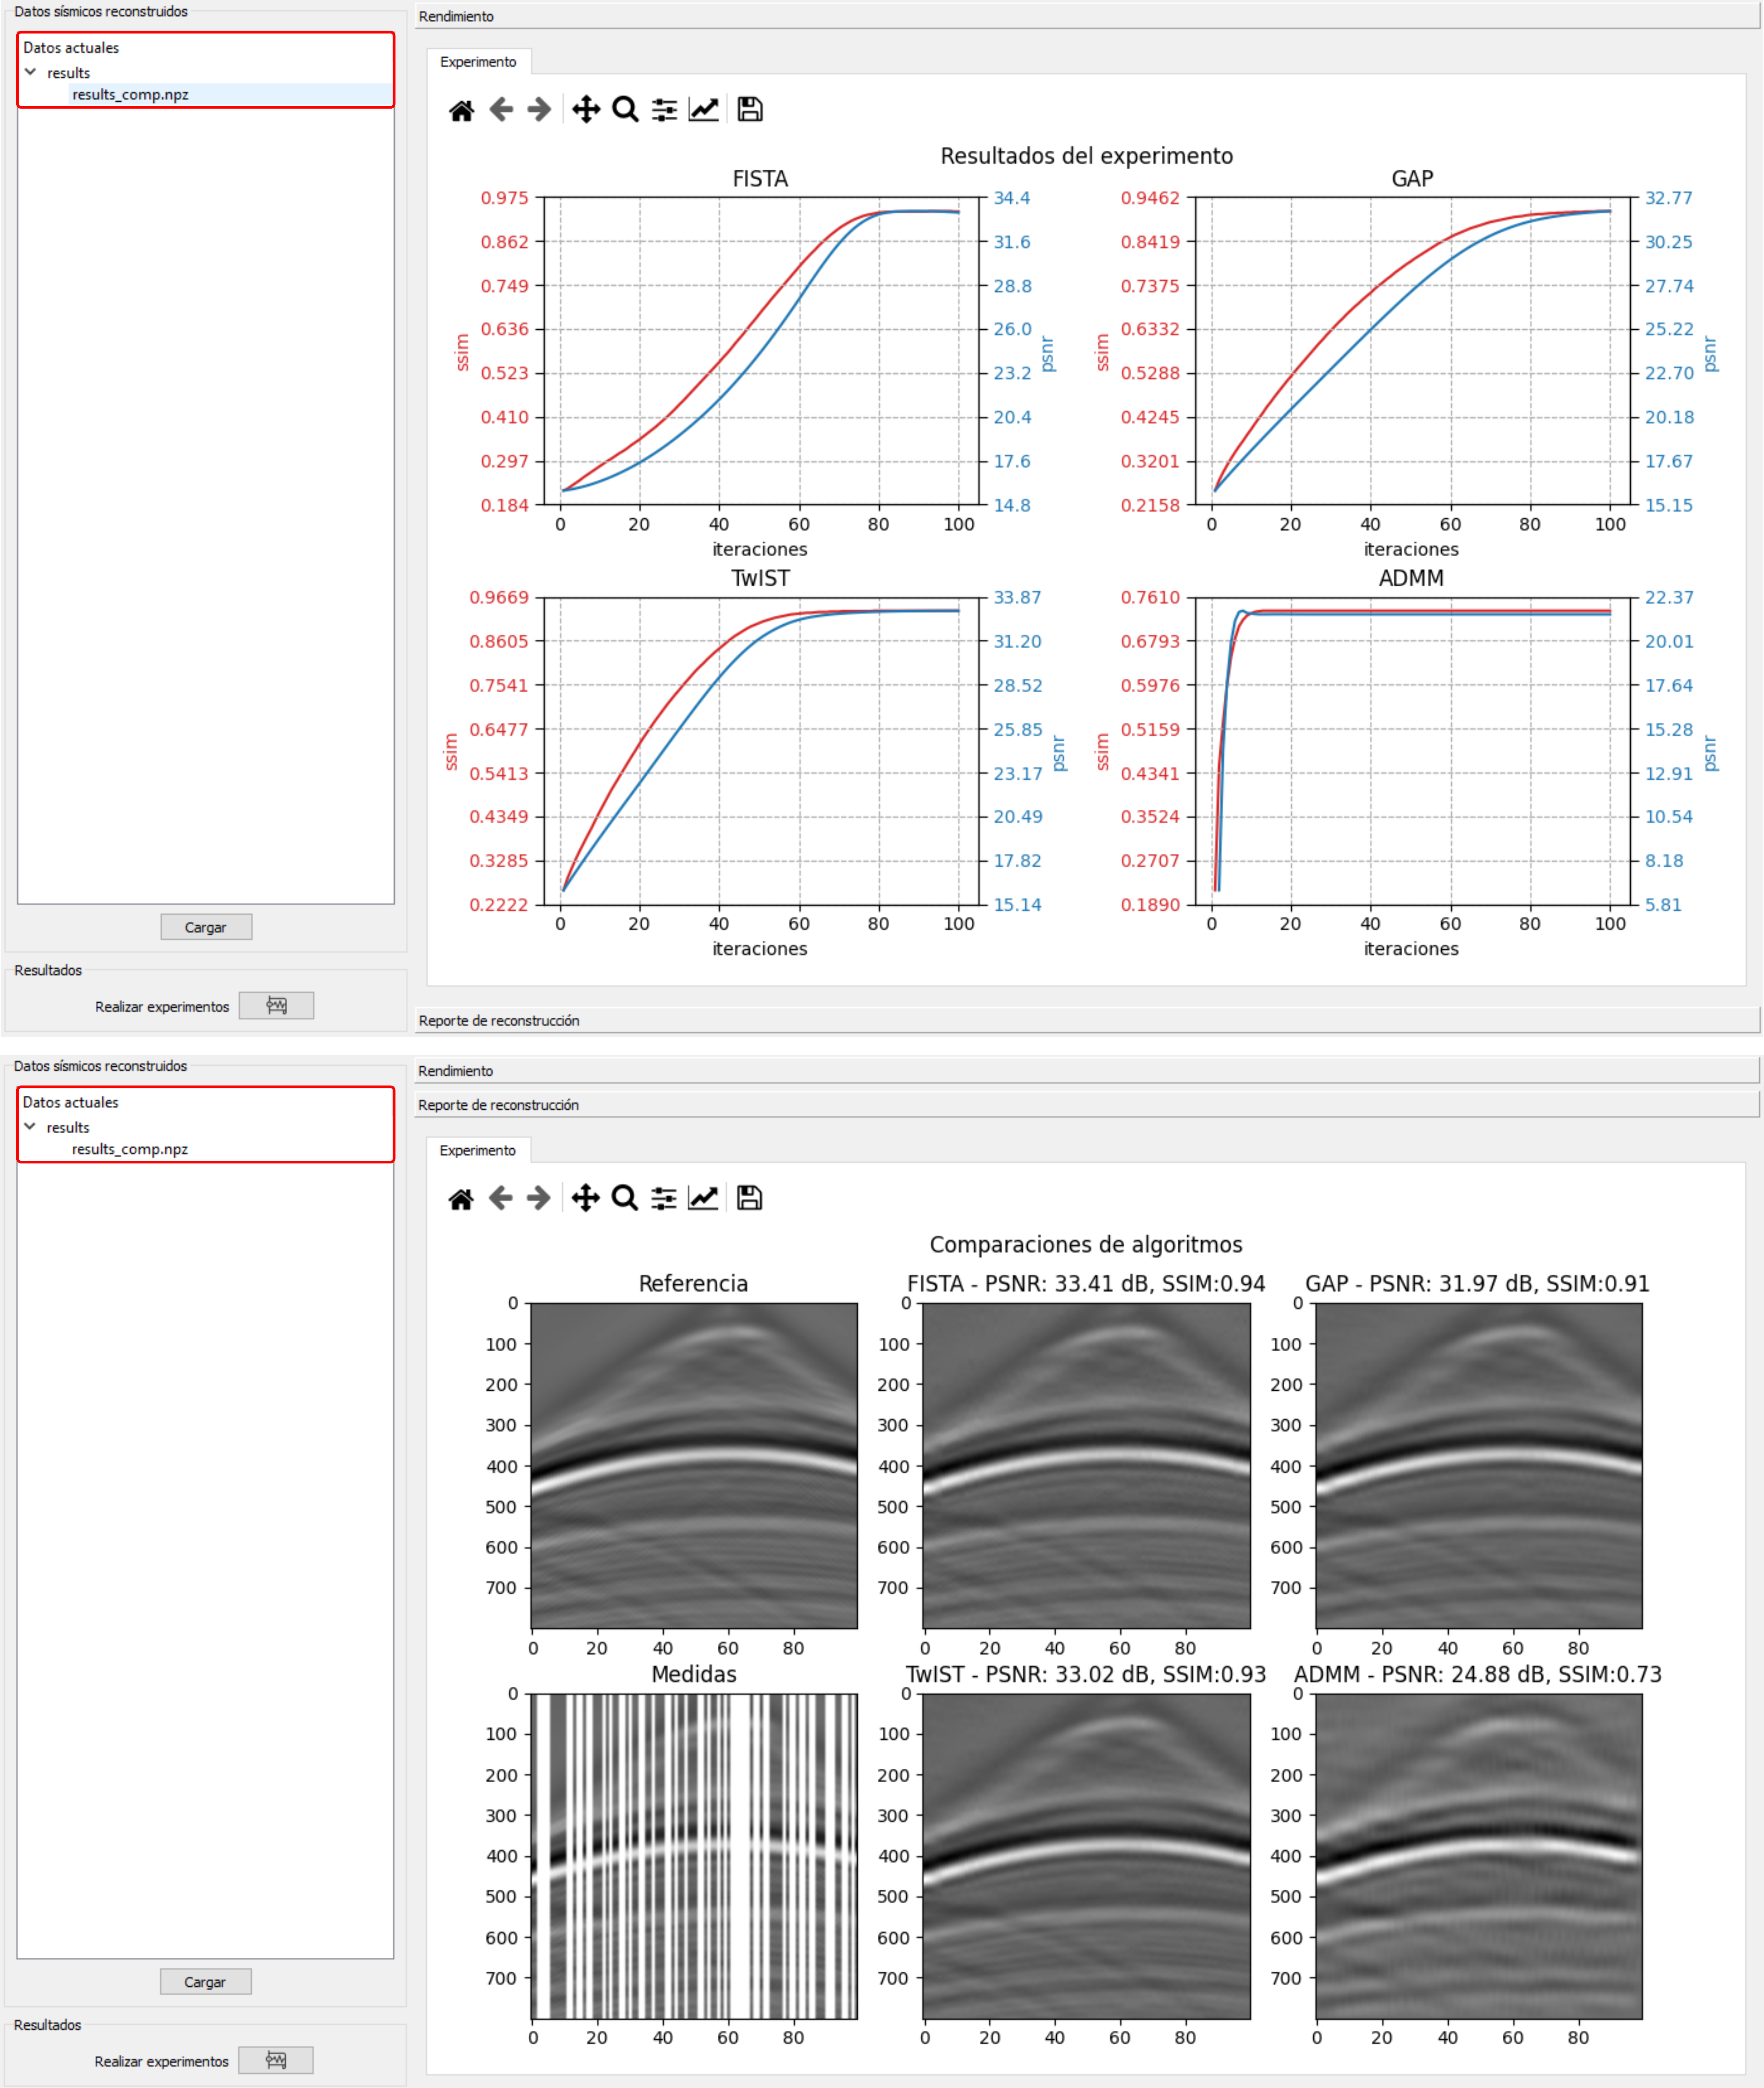
\includegraphics[width=1\linewidth]{report-6.png}
	\captionof{figure}{Visualización de los resultados la comparación de algoritmos.}
	\label{fig:report_6}
\end{Figure}

\newpage
\section{Módulo ReDs - Reconstrucción de Disparos (RD)}

El módulo ReDS-RD (reconstrucción de disparos) realiza la estimación de disparos sísmicos completos, faltantes en la adquisición, usando algoritmos de gradiente descendiente que aprovechan representaciones escasas de los datos en dominios transformados como Curvelet, DCT y Wavelets.

\newpage
\section{Acerca de}

Como se mencionó al principio de este manual, esta aplicación se encuentra asociada con varias compañias colombianas relacionadas en el sector de la sísmica. Por lo tanto, si se pulsa el botón \emph{Acerca de}, como se muestra en la figura \ref{fig:about_tab}, se abrirá una nueva ventana donde se menciona dicha información de manera más detallada, como se observa en la figura \ref{fig:about_of}.

\begin{Figure}
    \centering
    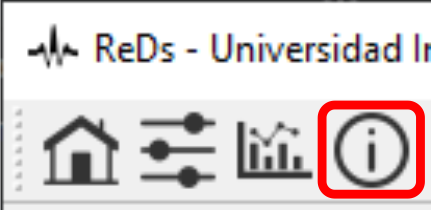
\includegraphics[width=0.25\linewidth]{about-tab.png}
    \captionof{figure}{Botón de Acerca de.}
    \label{fig:about_tab}
\end{Figure}

\begin{Figure}
    \centering
    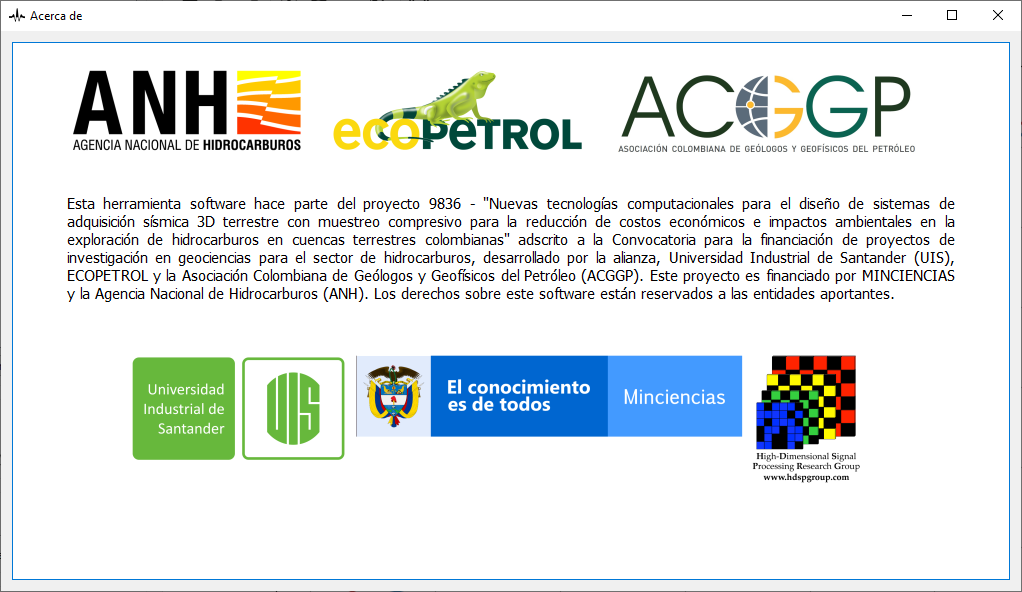
\includegraphics[width=1\linewidth]{about.png}
     \captionof{figure}{Acerca de.}
    \label{fig:about_of}
\end{Figure}

\section{Recomendaciones de uso}

Con el propósito de obtener el mayor rendimiento de la aplicación se realizan las siguientes recomendaciones:

\begin{itemize}[leftmargin=0.5in]
	\setlength\itemsep{0em} 
    \item Realizar los experimentos siguiendo este orden:
    
    \textbf{Menú principal}
    
    \begin{enumerate}[leftmargin=0.5in]
    	\setlength\itemsep{0em} 
        \item Cargar un dato sísmico.
        \item Seleccionar el algoritmo que desea usar y configurar sus parámetros.
        \item Seleccionar el tipo de submuestreo y configurar sus parámetros.
        \item Darle un nombre a los resultados a guardar usando el botón \hspace{0.5mm} \faSave.
        \item Inicial el experimento usando el botón \hspace{0.5mm} \faPlay.
    \end{enumerate}
    
    \textbf{Ajuste de parámetros}
    
    Se sigue el mismo orden que el menú principal, pero los incisos 2 y 3 cambian por:
    
    \begin{enumerate}[leftmargin=0.5in]
    	\setlength\itemsep{0em} 
        \item[2.] Seleccionar el algoritmo que desea usar y configurar la cantidad máxima de iteraciones.
        \item[3.] Configurar el ajuste de parámetros que se desea realizar.
    \end{enumerate}
    
    \item Para la configuración de parámetros se recomienda usar valores razonables y no excesivamente grandes debido a que dependiendo del equipo de cómputo utilizado y al algoritmo seleccionado, se puede elevar el consumo de CPU y memoria RAM al intentar utilizar otras herramientas de la aplicación mientras se corre algún experimento. Actualmente, la aplicación continúa en desarrollo para soportar estos tipos de usos o genera mensajes de advertencia al usuario.
    
\end{itemize}


% \begin{thebibliography}{99}
% \bibitem{web1} \url{http://bit.ly/PhysLab_Link01}
% \bibitem{web2} \url{http://bit.ly/PhysLab_Link02}
% \end{thebibliography}
\end{document}